\documentclass[a4paper,10pt,oneside]{article}
\usepackage[polutonikogreek,italian]{babel}
\usepackage[utf8x]{inputenc}
\usepackage{amsmath}
\usepackage{amsthm}
\usepackage{amssymb}
\usepackage{amscd}
\usepackage{graphicx}
\usepackage{float}
\usepackage{array}
\usepackage{rotating}
\usepackage[small]{caption}
\usepackage{lscape}
\usepackage{fancybox}
\usepackage{booktabs}
\parindent0ex 
\renewcommand{\fboxsep}{0.5cm}
\usepackage{hyperref}
\renewcommand{\textfraction}{0.05}
\renewcommand{\topfraction}{0.95}
\renewcommand{\bottomfraction}{0.95}
\renewcommand{\floatpagefraction}{0.35}
\setcounter{totalnumber}{5}
\restylefloat{figure}
\newlength{\drop}
\begin{document}

\begin{center}
{\huge Laboratorio di acustica}
\end{center}

\begin{abstract}
In questo laboratorio ripeteremo l'esperimento di Kundt del 1866\footnote{L'articolo originale è stato pubblicato su\emph{Annalen der Physik} (Leipzig: J. C. Poggendorff) 127 (4): p.497–523. ed è disponibile gratuitamente su \url{http://books.google.com}} avvalendoci di una strumentazione più moderna che ci permetterà di effettuare delle osservazioni e delle misure impossibili ai tempi dello sperimentatore originale. Misureremo la velocità del suono, la lunghezza acustica di un tubo e la disposizione spaziale delle striature che si vengono a formare nella polvere di sughero a causa della risonanza. Avvalendoci di generatori ad ultrasuoni studieremo anche l'interferenza e la diffrazione del suono da parte di ostacoli di varia forma.
\end{abstract}

\vspace{3cm}





\section*{Lo specchio di LLoyd}

In questo esperimento analizzeremo l'interferenza tra due onde sonore ultrasoniche, una ottenuta direttamente dal trasduttore ultrasonico l'altra per riflessione della prima su uno specchio metallico. Le due onde interferiranno distruttivamente o costruttivamente nella posizione del ricevitore ultrasonico in funzione della distanza $d$ dello specchio dall'asse che congiunge i trasduttori.
\begin{figure}[H]
 \centering
 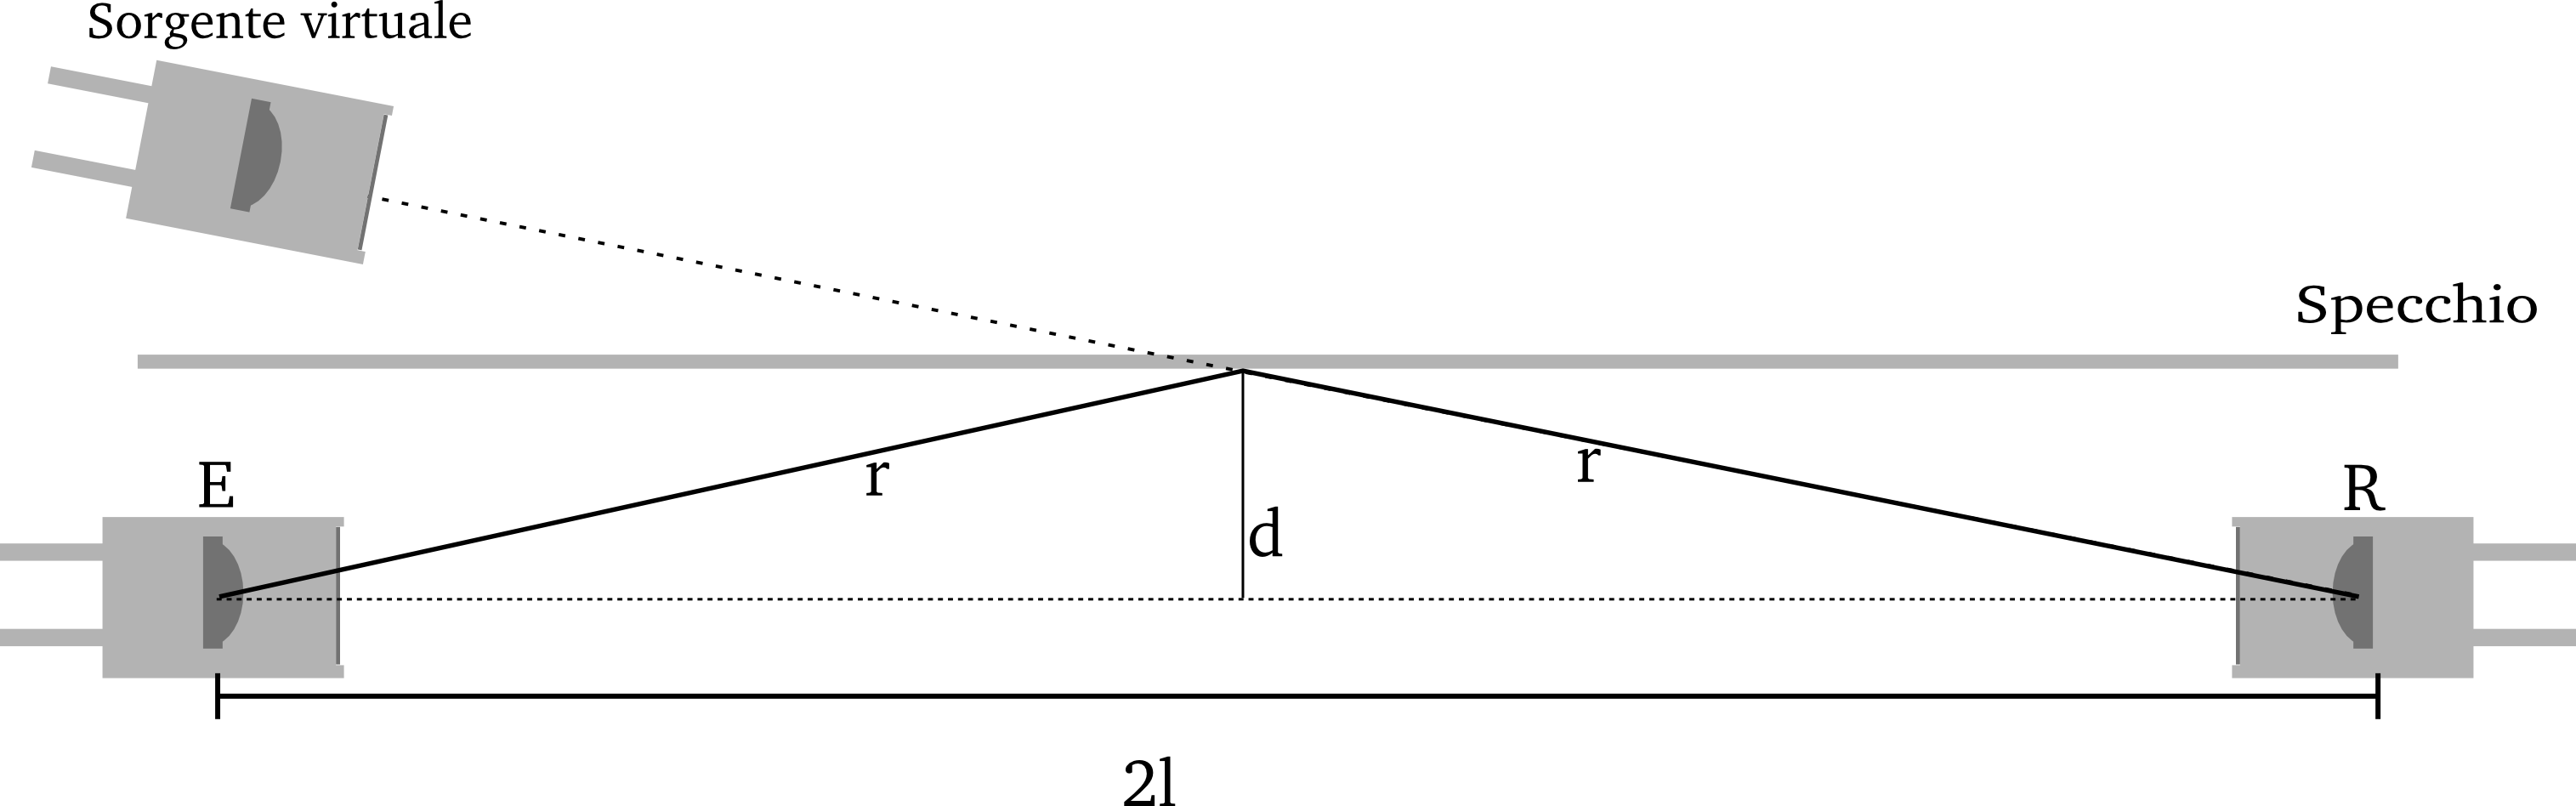
\includegraphics[width=\textwidth]{../Immagini/lloyd1.png}
 % lloyd1.png: 3208x652 pixel, 288dpi, 28.34x5.76 cm, bb=0 0 803 163
 \caption{Disposizione sperimentale dei trasduttori ultrasonici e dello specchio metallico}
 \label{fig:llody1}
\end{figure}

Utilizzando le notazioni di figura [\ref{fig:llody1}] e ricordando che due onde,inizialmente in fase, interferiscono costruttivamente se la differenza di cammino è pari ad un numero intero di lunghezze d'onda e distruttivamente se tale differenza è pari ad un numero dispari di mezze lunghezze d'onda possiamo scrivere:
\begin{equation}\label{max}
 k\lambda=2r-2l
\end{equation}
per i massimi e
\begin{equation}\label{min}
 \frac{2k+1}{2}\lambda=2r-2l
\end{equation}
per i minimi.
Se introduciamo nelle due relazioni [\ref{max}] e [\ref{min}] la distanza $d$ dello specchio dall'asse che congiunge i centri di emettitore e ricevitore possiamo scrivere:
\begin{equation}\label{lloyd_dmax}
  d=\sqrt{\frac{k^2\lambda^2}{4}+lk\lambda}
\end{equation}
per i massimi e
\begin{equation}\label{llody_dmin}
 d=\sqrt{\left(\frac{2k+1}{4}\right)^2\lambda^2+\frac{2k+1}{2}\lambda l}
\end{equation}
per i minimi. Come possiamo, tramite questo esperimento, capire che le onde sonore sono longitudinali e non trasversali?
Nei calcoli sopra svolti si è ipotizzato che ricevitore ed emettitore siano puntiformi, i trasduttori reali hanno una dimensione finita per cui il comportamento che osserveremo in laboratorio si discosterà da quello ideale qui analizzato.

\section*{Interferenza e diffrazione di onde sonore}

Nella seconda esperienza con gli ultrasuoni  analizzeremo l'interferenza e la diffrazione di onde sonore ultrasoniche da parte di ostacoli rigidi. Come primo caso studieremo l'interferenza da due fenditure di larghezza inferiore alla lunghezza d'onda del suono incidente. Affinché in un punto sulla circonferenza di raggio $r$, su cui giace il ricevitore, la differenza tra i cammini acustici delle onde irradiantisi sia pari ad un numero dispari di mezze lunghezze d'onda, dovrà valere la condizione:
\begin{equation}
 r'-r''=\frac{2k+1}{2}\lambda
\end{equation}

ovvero utilizzando la notazione di figura [\ref{fig:young_schema}]:
\begin{equation}\label{young_completa}
 \sqrt{r^2\cos^2\theta+(r\sin\theta-\frac \delta 2)^2}-\sqrt{r^2\cos^2\theta+(r\sin\theta+\frac \delta 2)^2}=\frac{2k+1}{2}\lambda
\end{equation}
che possiamo riscrivere come:
\begin{equation}\label{young_semplif}
 \sqrt{1+\frac{\delta}{4r^2}-\frac{\delta\sin\theta}{r}}-\sqrt{1+\frac{\delta}{4r^2}+\frac{\delta\sin\theta}{r}}=\frac{2k+1}{2r}\lambda
\end{equation}
possiamo approssimare la [\ref{young_semplif}] utilizzando uno strumento matematico noto come espansione in serie di Maclaurin\footnote{Utilizzeremo il fatto che per $|x|<1$ è possibile utilizzare l'approssimazione $\sqrt{1+x}=1+\frac 1 2 x -\frac 1 8 x^2 +\frac{1}{16} x^3+\ldots$}:
\begin{equation}\label{young_approx1}
 \delta\sin\theta=\frac{2k+1}{2}\lambda
\end{equation}

dove si sono presi unicamente i termini di primo grado nell'espansione in serie. I minimi di intensità lungo la semicirconferenza riportata in figura [\ref{fig:young_schema}] saranno quindi approssimativamente distribuiti angolarmente secondo l'equazione [\ref{young_approx1}]. L'approssimazione che abbiamo utilizzato è tanto più buona quanto più grande diventa il raggio $r$, sapreste ricavare una formula approssimata utilizzando fino ai termini quadratici dello sviluppo di Maclaurin della radice? Quanti minimi si potranno osservare al massimo nel caso di ultrasuoni con frequenza di $\sim 40kHz$ e distanza tra le fenditure pari a $3cm$? Per quale motivo si è scelto di muovere il ricevitore lungo una semicirconferenza?


\begin{figure}[H]
 \centering
 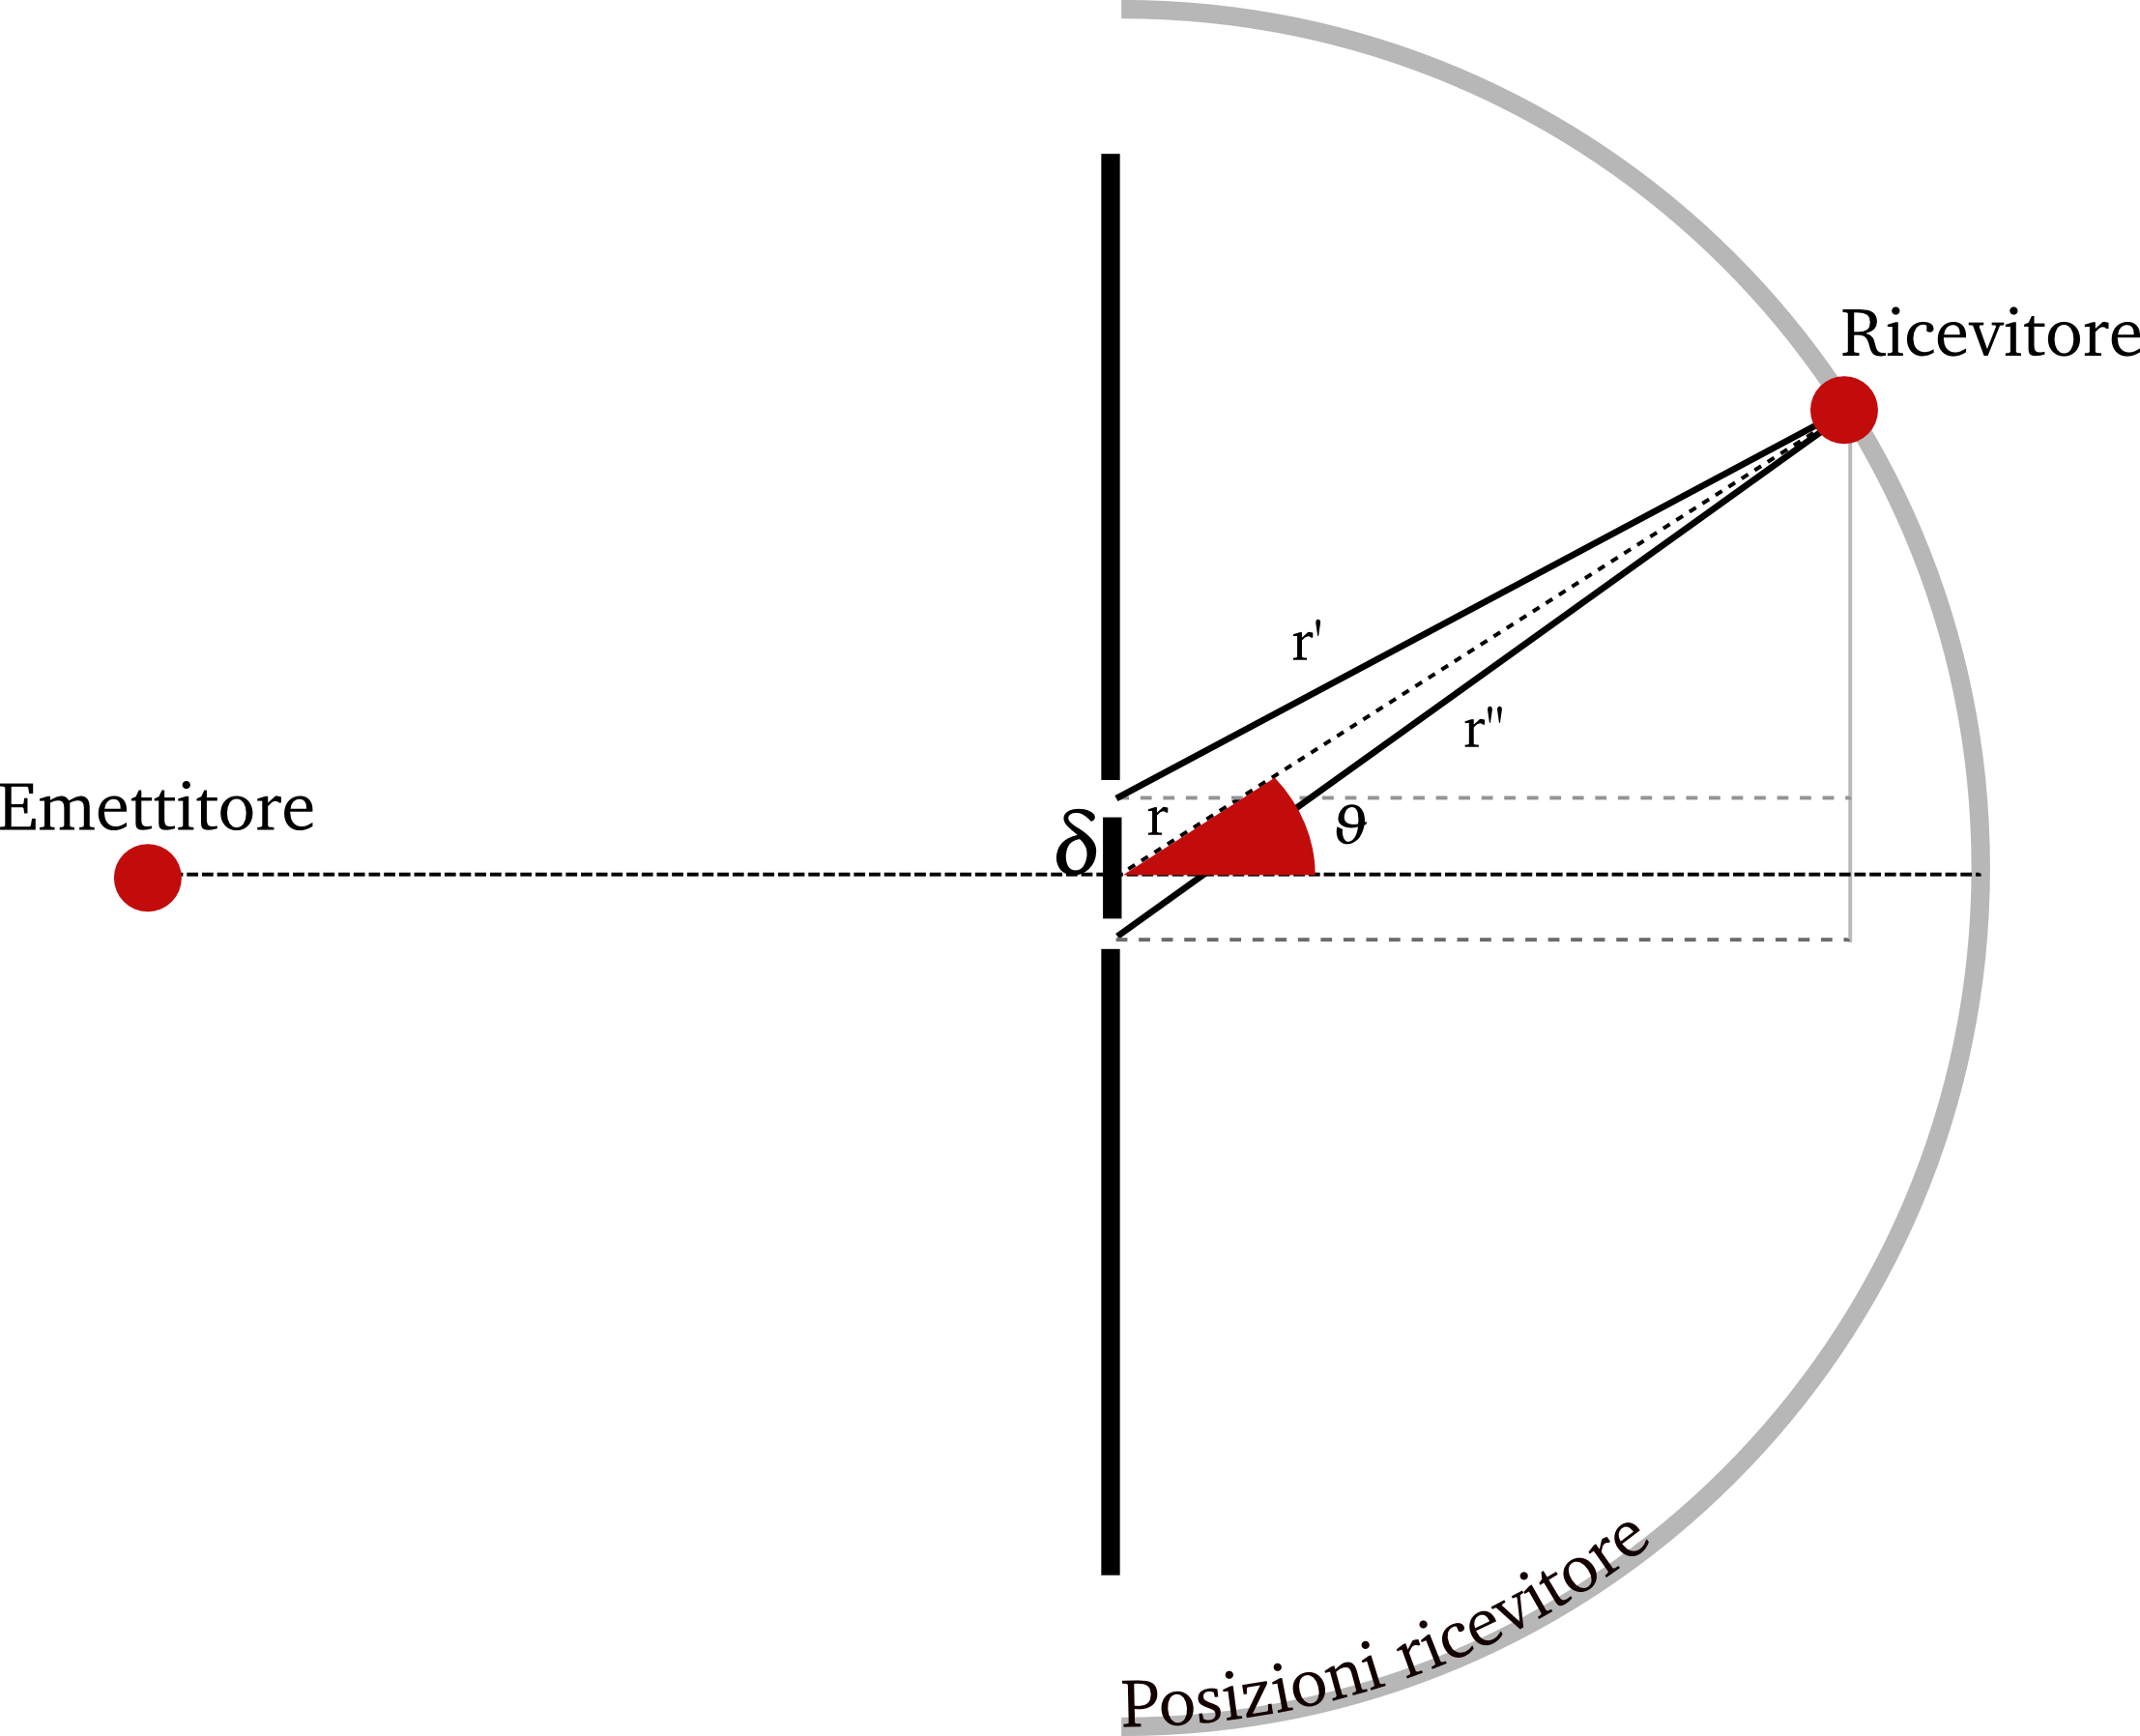
\includegraphics[width=\textwidth]{../Immagini/young.png}
 % young.png: 2214x1796 pixel, 600dpi, 9.37x7.60 cm, bb=0 0 266 215
 \caption{Interferenza tra due fenditure di larghezza inferiore alla lunghezza d'onda degli ultrasuoni incidenti}
 \label{fig:young_schema}
\end{figure}


Nel secondo caso che analizzeremo  osserveremo la diffrazione degli ultrasuoni da parte di una fenditura di larghezza superiore alla lunghezza d'onda del suono incidente. Come avrete già studiato in classe possiamo individuare due comportamenti limite quello di Fraunhofer e quello di Fresnel, nel primo caso la distanza del ricevitore sarà grande rispetto alla larghezza della fenditura nel secondo caso invece il ricevitore si troverà ad una distanza dalla fenditura piccola rispetto alla larghezza di questa.
\begin{figure}[H]
 \centering
 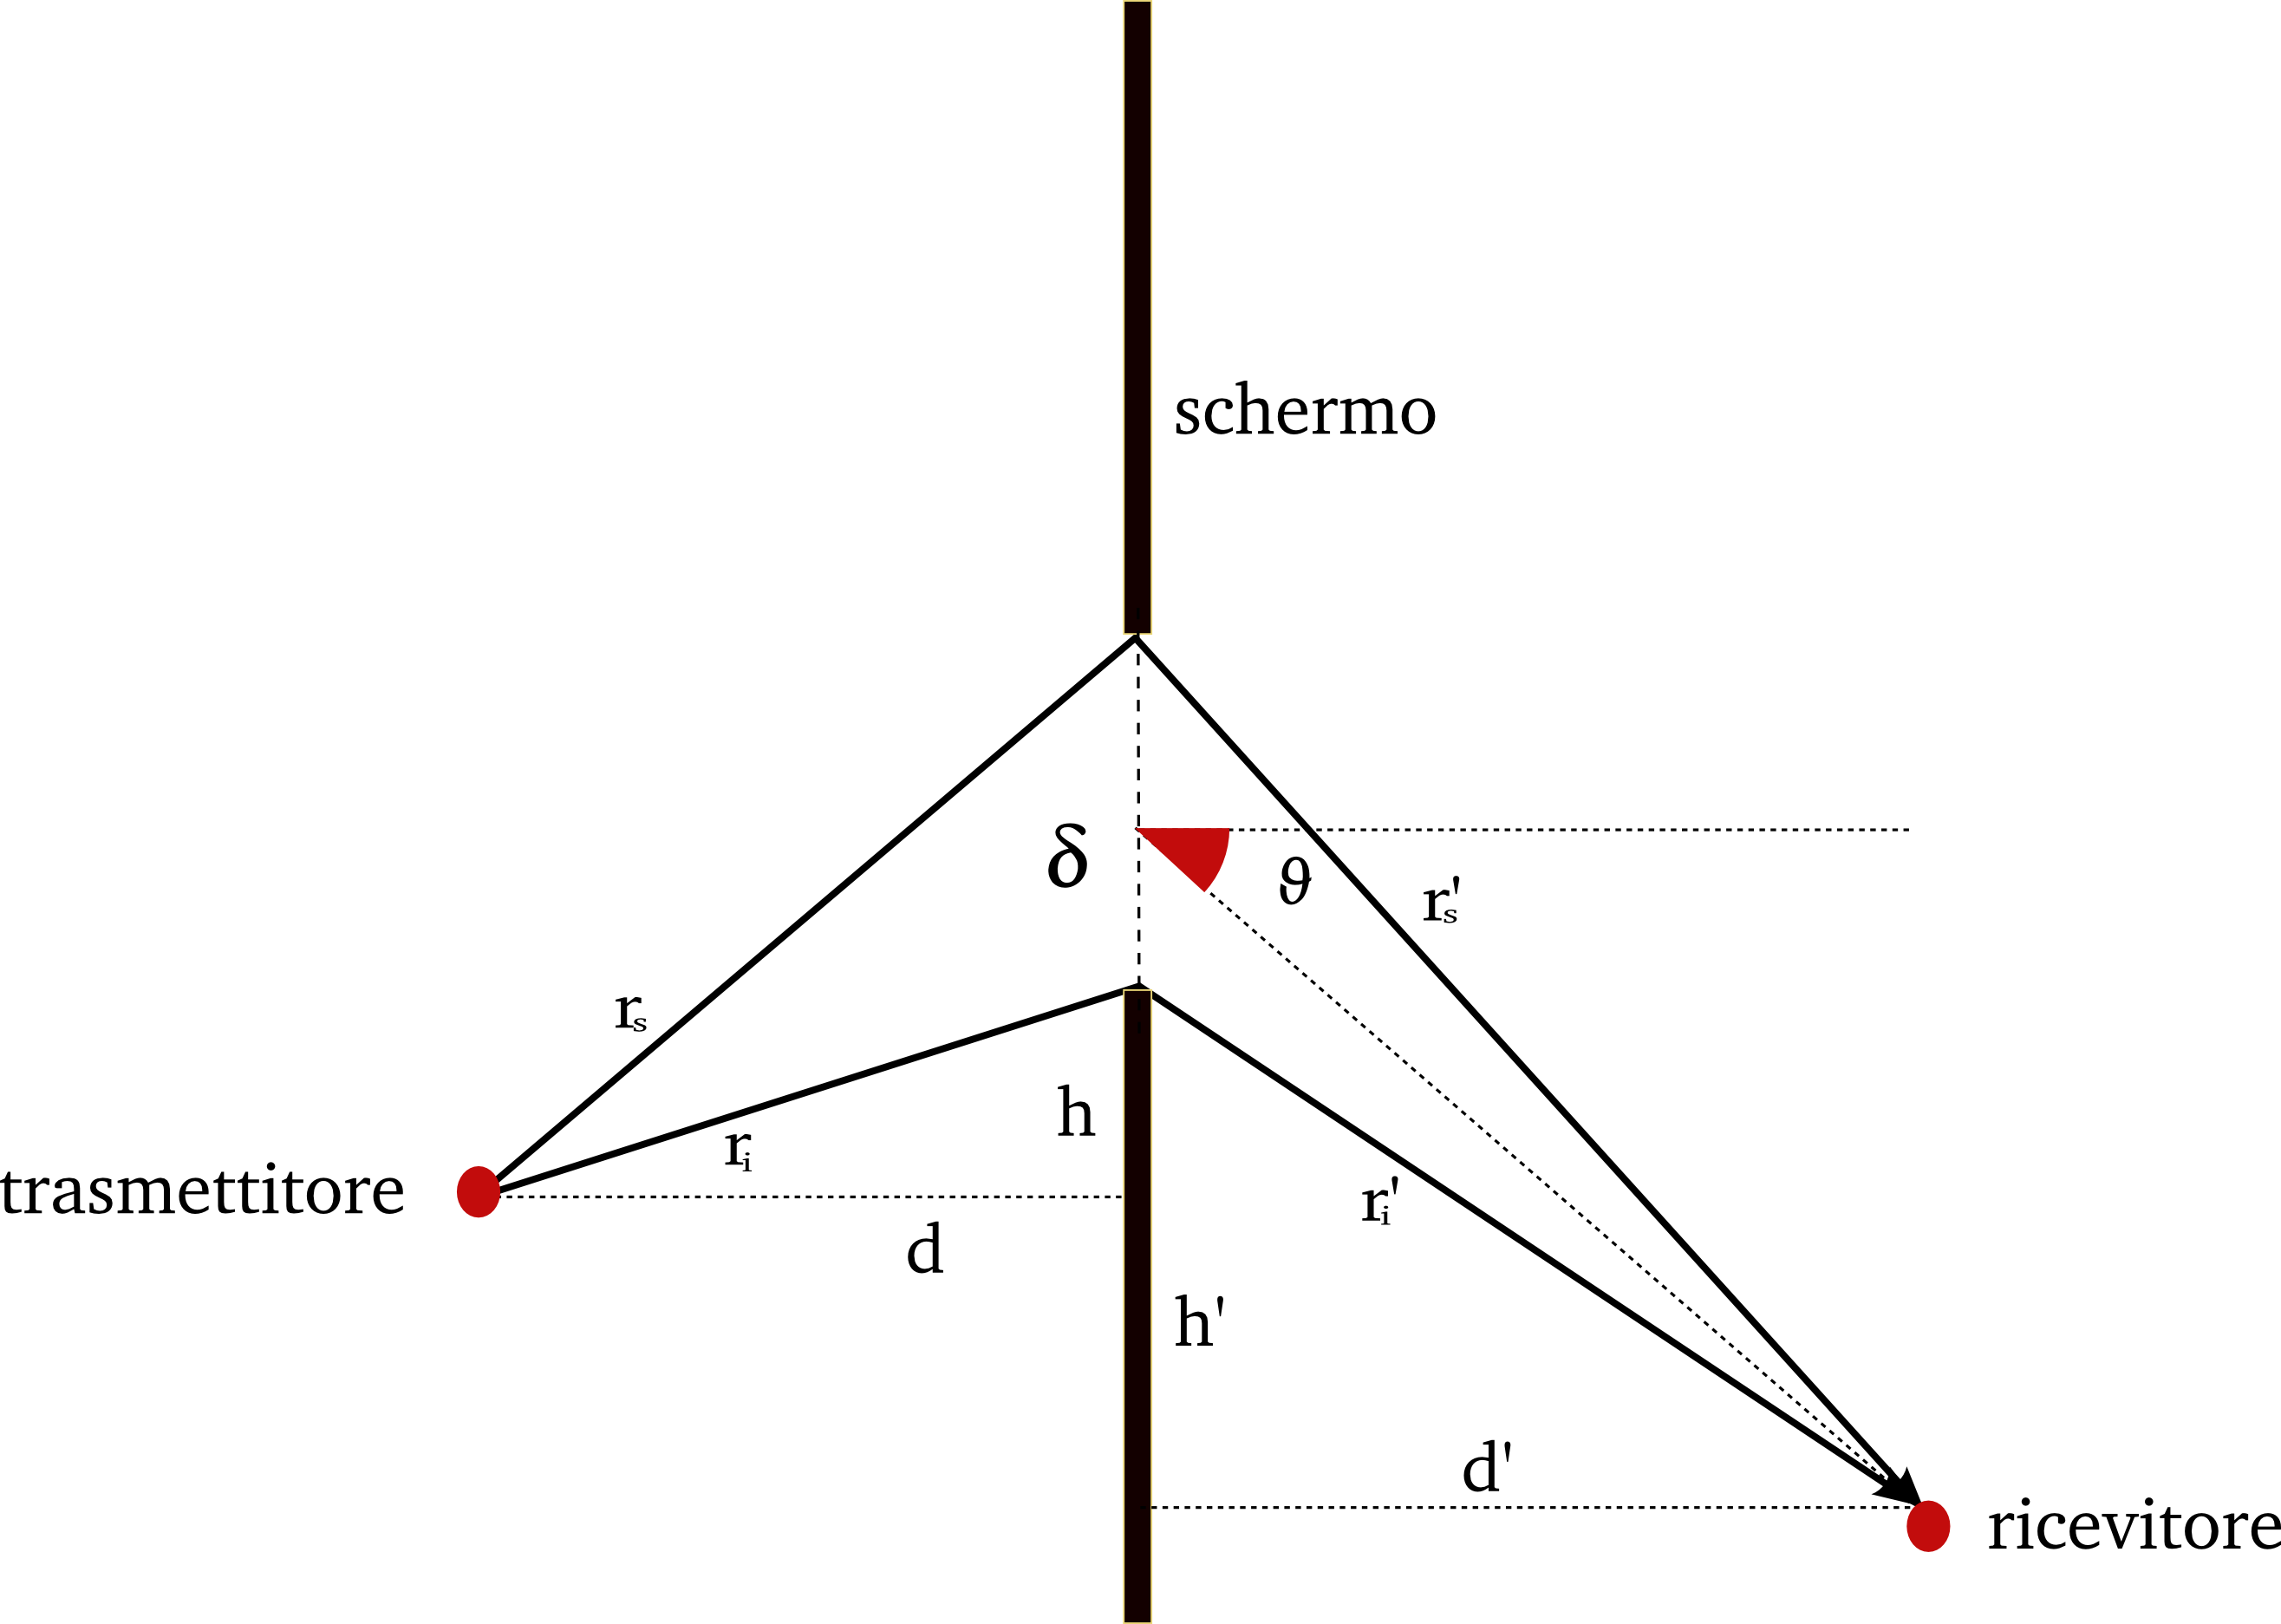
\includegraphics[width=\textwidth]{../Immagini/fraun.png}
 % fraun.png: 2631x1873 pixel, 288dpi, 23.24x16.55 cm, bb=0 0 659 469
 \caption{Per poter utilizzare l'approssimazione di onda piana dovrà essere $\frac 1 2(\frac 1 d+\frac{1}{d'})\delta \ll\lambda$}
 \label{fig:fraunuh}
\end{figure}
Per cercare di rendere quantitativo il discorso precedente facciamo ricorso allo schema di figura [\ref{fig:fraunuh}].
Calcoliamo la differenza di cammino acustico tra il tracciato superiore ed il tracciato inferiore che indicheremo con $\Delta$:
\begin{equation}
\Delta=\sqrt{d^2+(h+\delta)^2}+\sqrt{d'^2+(h'+\delta)^2}-\sqrt{d^2+h^2}-\sqrt{d'^2+h'^2} 
\end{equation}
applicando l'espansione in serie di Maclaurin come fatto nel caso dell'interferenza dalle due fenditure otteniamo:
\begin{equation}
 \Delta=\left(\frac h d+ \frac{h'}{d'}\right)\delta +\frac 1 2 \left(\frac{1}{d}+\frac{1}{d'}\right)\delta^2+\ldots
\end{equation}

se vale la condizione:
\begin{equation}
 \frac 1 2 \left(\frac{1}{d}+\frac{1}{d'}\right)\delta^2\ll \lambda
\end{equation}
allora l'onda incidente può essere considerata un'onda piana e ci troviamo nella condizione di Fraunhofer se invece
\begin{equation}
 \frac 1 2 \left(\frac{1}{d}+\frac{1}{d'}\right)\delta^2\geq 1
\end{equation}
l'onda incidente non può essere considerata piana e il sistema deve essere analizzato con la più complessa teoria di Fresnel sulla diffrazione. Nel caso di Fraunhofer la condizione per il minimo di intensità della figura di diffrazione è:
\begin{equation}
 \delta \sin\theta=k\lambda,\quad k=\pm 1,\pm 2,\ldots
\end{equation}

Quali dovranno essere i valori di $d'$, $d$ e $\delta$ per poter applicare l'approssimazione di Fraunhofer nel caso di un onda incidente di frequenza $\nu=40kHz$? 


\section*{Onde stazionarie nei tubi}

Durante questa esperienza genereremo delle onde stazionarie che, come avete già studiato, nascono dall'interferenza costruttiva di due onde progressive con velocità opposte, nel nostro caso un'onda incidente generata da un altoparlante ed un onda riflessa dalle estremità del tubo.

Considereremo due casi:
\begin{itemize}
 \item Tubo aperto
\item Tubo semichiuso
\end{itemize}

Prendiamo come esempio il tubo semichiuso:
\begin{figure}[H]
 \centering
 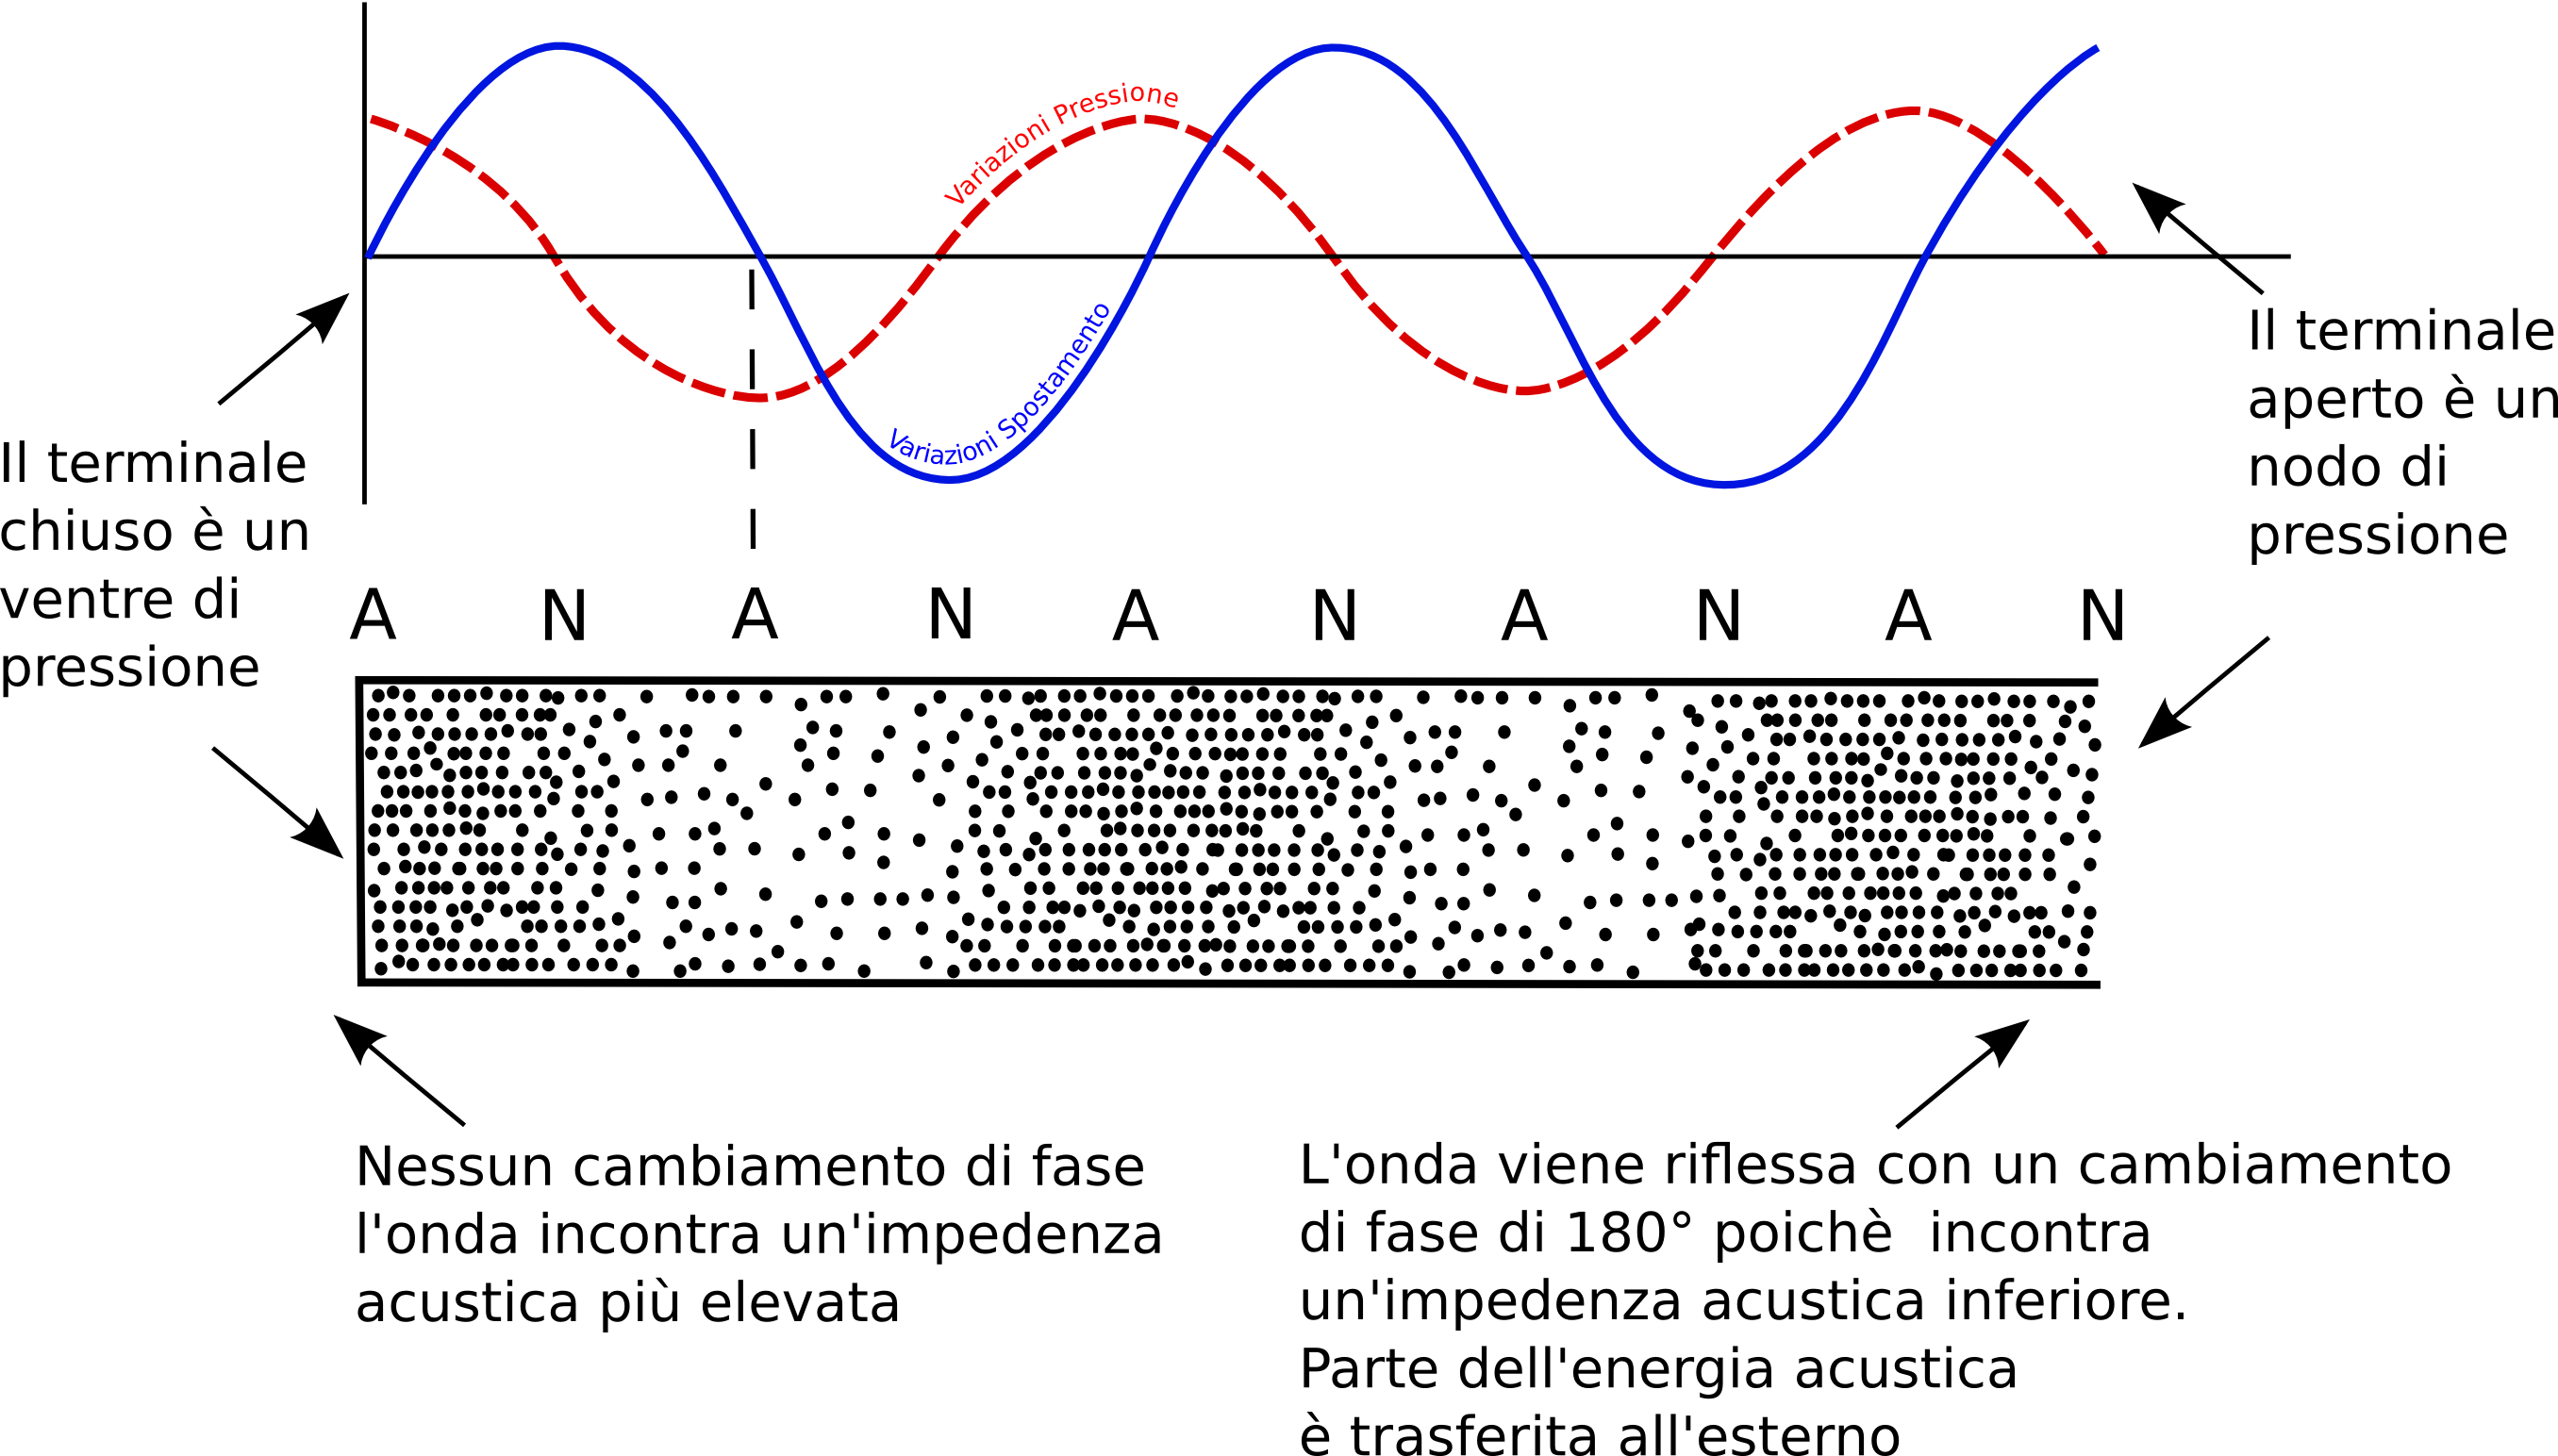
\includegraphics[width=1.1\textwidth]{../Immagini/tubo_semichiuso.png}
 % tubo_semichiuso.png: 2746x1564 pixel, 304dpi, 22.95x13.07 cm, bb=
 \caption{Onda stazionaria all'interno di un tubo semichiuso}
 \label{fig:tubo_semichiuso}
\end{figure}
vediamo che all'estremità chiusa l'onda sonora si riflette senza cambiamenti di fase mentre all'estremità aperta vi è un cambiamento di fase di $\pi$. La diversa riflessione dell'onda da parte dell'estremità aperta e di quella chiusa è la causa delle differenti frequenze risonanti nei due casi.

\subsection*{Tubo aperto}
Ricordiamo che nel tubo aperto le lunghezze d'onda per cui un tubo  di lunghezza $L$ risuona sono date da:
\begin{equation}\label{aperto_1}
 \lambda_k=\frac{2L}{k}\qquad k=1,2,3...
\end{equation}

mentre per una data lunghezza d'onda $\lambda$ le lunghezze risonanti saranno:
\begin{equation}\label{aperto_2}
 L_k=k\frac{\lambda}{2}\qquad k=1,2,3... 
\end{equation}

ovvero utilizzando la relazione $\lambda=v/\nu$ possiamo riscrivere le relazioni [\ref{aperto_1}] e [\ref{aperto_2}] come:
\begin{equation}
 \nu_k=k\frac{v}{2L}
\end{equation}
e
\begin{equation}
 L_k=k\frac{v}{2\nu}
\end{equation}

Utilizzando un tubo aperto della lunghezza di $0.60m$ otteniamo teoricamente\footnote{Si può dimostrare che un tubo aperto si comporta come se fosse più lungo al fine della determinazione della frequenza risonante} le seguenti frequenze risonanti:


\begin{table}[H]
\begin{center}
\begin{tabular}{lll}\toprule
$Armonica$ &$k$&$\nu$\\ \midrule
Prima & 1 & 283Hz\\
Seconda & 2&567Hz\\
Terza & 3&851Hz\\
\ldots &\ldots&\ldots \\ \bottomrule
\end{tabular}\caption{Le frequenze sono state calcolate utilizzando per la velocità del suono in aria il valore $340.0ms^{-1}$}\label{tab:aperto}
\end{center}
\end{table}


\begin{figure}[H]
 \centering
 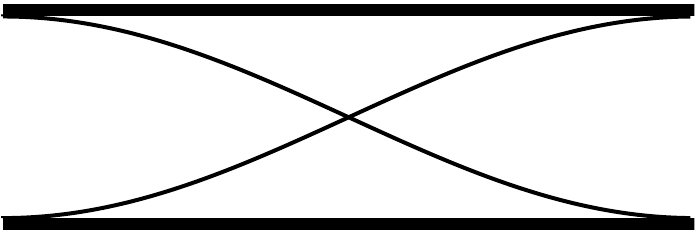
\includegraphics[width=\textwidth]{../Immagini/aperto_1.png}
 % aperto_1.png: 696x234 pixel, 90dpi, 19.64x6.60 cm, bb=
 \caption{Armonica fondamentale del tubo aperto, nella figura è rappresentata l'onda di spostamento notiamo la presenza di un unico nodo al centro}
 \label{fig:aperto_fondamentale}
\end{figure}

\begin{figure}[H]
 \centering
 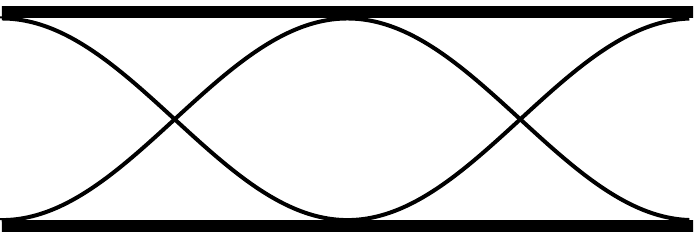
\includegraphics[width=\textwidth]{../Immagini/aperto_2.png}
 % aperto_2.png: 696x238 pixel, 90dpi, 19.64x6.72 cm, bb=
 \caption{Seconda armonica nel tubo aperto, nella figura è rappresentata l'onda di spostamento. Notiamo la presenza di due nodi}
 \label{fig:aperto_seconda}
\end{figure}



\subsection*{Tubo semichiuso}
Le frequenze risonanti per il tubo semichiuso sono diverse e risultano:
\begin{equation}\label{chiuso_1}
 \lambda_k=\frac{4L}{2k+1}\qquad k=0,1,2..
\end{equation}

mentre per una lunghezza d'onda data:
\begin{equation}\label{chiuso_2}
 L_k=(2k+1)\frac{\lambda}{4}\qquad k=0,1,2..
\end{equation}

esprimendo le relazioni [\ref{chiuso_1}] e [\ref{chiuso_2}] in funzione delle frequenza otteniamo:

\begin{equation}
 \nu_k=(2k+1)\frac{v}{4L}
\end{equation}

e
\begin{equation}
 L_k=(2k+1)\frac{v}{\nu}
\end{equation}


utilizzando un tubo semichiuso della lunghezza di $0.60m$\footnote{Anche in questo caso le frequenze calcolate con questa formula sono unicamente dei valori approssimati} otteniamo ad esempio le frequenze risonanti:
\begin{table}[H]
\begin{center}
\begin{tabular}{lll}\toprule
$Armonica$ &$k$&$\nu$\\ \midrule
Prima & 0 & 142Hz\\
Seconda & 1&425Hz\\
Terza & 2&568Hz\\
\ldots &\ldots&\ldots \\ \bottomrule
\end{tabular}\caption{Le frequenze sono state calcolate utilizzando per la velocità del suono in aria il valore $340.0ms^{-1}$}\label{tab:chiuso}
\end{center}
\end{table}

\begin{figure}[H]
 \centering
 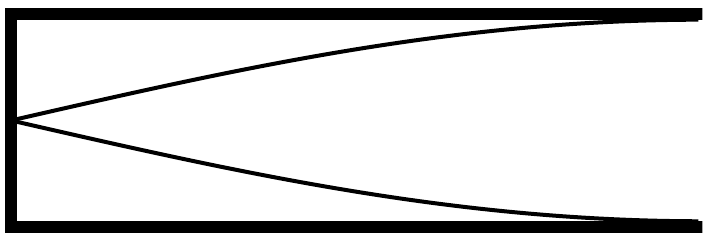
\includegraphics[width=\textwidth]{../Immagini/chiuso_1.png}
 % chiuso_1.png: 706x240 pixel, 90dpi, 19.93x6.77 cm, bb=
 \caption{Armonica fondamentale del tubo semichiuso, nella figura è rappresentata l'onda di spostamento notiamo la presenza di un nodo}
 \label{fig:chiuso_base}
\end{figure}

\begin{figure}[H]
 \centering
 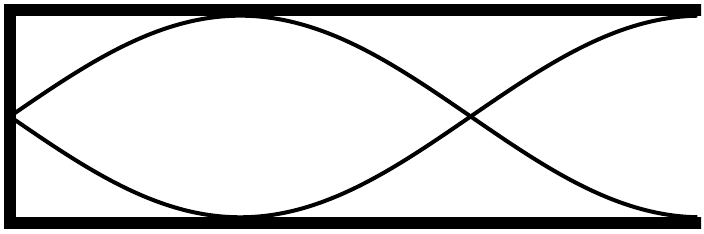
\includegraphics[width=\textwidth]{../Immagini/chiuso_2.png}
 % chiuso_2.png: 704x234 pixel, 90dpi, 19.87x6.60 cm, bb=
 \caption{Seconda armonica del tubo semichiuso, notiamo la presenza di due nodi. In figura è rappresentata l'onda di spostamento}
 \label{fig:chiuso_seconda}
\end{figure}


\subsection*{Calcolo della velocità del suono}
Utilizzando le formule per il tubo semichiuso possiamo misurare in maniera estremamente semplice la velocità del suono. Calcoliamo la differenza tra due lunghezze risonanti ad una data lunghezza d'onda $\lambda$:
\begin{equation}
 L_{k+1}-L_k=[2(k+1)+1]\frac{\lambda}{4}-(2k+1)\frac{\lambda}{4}=\lambda/2
\end{equation}
misurando due di tali lunghezze successive ad una data frequenza possiamo quindi ottenere il valore di mezza lunghezza d'onda.
Ricordando che:
\begin{equation}
 \lambda=vT
\end{equation}
dove $T$ è il periodo dell'onda:
\begin{equation}
 T=\frac{1}{\nu}
\end{equation}
possiamo ricavare:
\begin{equation}
 v=\lambda\nu
\end{equation}
ed ottenere la velocità del suono. Possiamo confrontare il valore misurato in laboratorio con il valore calcolato della velocità del suono in funzione della temperatura secondo la formula seguente:
\begin{equation}\label{sound_speed}
 v\sim 331.3\sqrt{\frac{T}{T_0}}\ ms^{-1}
\end{equation}
dove $T$ è la temperatura ambiente in Kelvin e $T_0=273,15K$.
 

\subsection*{Correzione per la lunghezza acustica}

La trattazione teorica elementare non tiene conto del fatto che la riflessione dell'onda sonora da parte dell'estremità aperta non è completa e che l'aria che esce dal tubo tende ad espandersi. Per questi motivi è estremamente facile accorgersi durante la sessione di laboratorio che le formule sopra citate non sono corrette, precisamente nel caso reale il tubo si comporta come se fosse leggermente più lungo per cui nel caso del tubo semichiuso avremo:


\begin{equation}
 L_k+\delta=(2k+1)\frac{\lambda}{4}
\end{equation}

mentre nel caso del tubo aperto:
\begin{equation}
 L_k+2\delta=k\frac{\lambda}{2}
\end{equation}

è possibile calcolare (Levine  e Schwinger, 1948) un valore per $\delta$ in funzione del diametro del tubo, tale calcolo è sfortunatamente estremamente complesso e non eseguibile con gli strumenti matematici disponibili alle scuole superiori. 
Durante l'esperimento dovremmo riuscire a misurare un valore prossimo a:
\begin{equation}
 \delta\sim 0.65r
\end{equation}

dove $r$ è il raggio del tubo.

\subsection*{Striature nella polvere di sughero}

Sin dai primi esperimenti di Kundt si notò come all'instaurarsi di un'onda progressiva all'interno del tubo comparissero delle striature nella polvere utilizzata per visualizzare i nodi e i ventri del modo risonante. L'origine di tali striature eluse per quasi 70 anni la comunità scientifica. Fu soltanto nella seconda metà del XX secolo che, con il diffondersi di sistemi più sofisticati per la raccolta dei dati, il fenomeno venne interpretato correttamente\footnote{C.Andreade Trans. Roy. Soc. (London) A230, 413 (1932) l'articolo originale è disponibile in biblioteca o sulla pagina web dedicata a questo esperimento all'indirizzo \url{http://cartan.e-moka.net}}.


\begin{figure}[H]
 \centering
 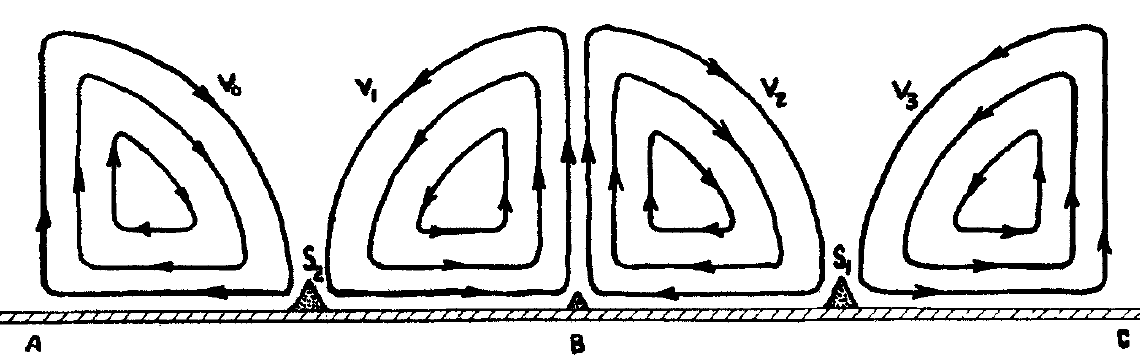
\includegraphics[width=\textwidth]{../Immagini/cork2.png}
 % cork2.png: 1140x363 pixel, 90dpi, 32.18x10.25 cm, bb=
 \caption{Rappresentazione dei vortici che generano le striature all'interno del tubo di Kundt}
 \label{fig:cork2}
\end{figure}

Empiricamente si è visto che la separazione $S$ tra due striature alla distanza $y$ da un ventre segue la regola:
\begin{equation}
 S=0.422\cos^{0.44}(2\pi y/\lambda)
\end{equation}


\begin{figure}[H]
 \centering
 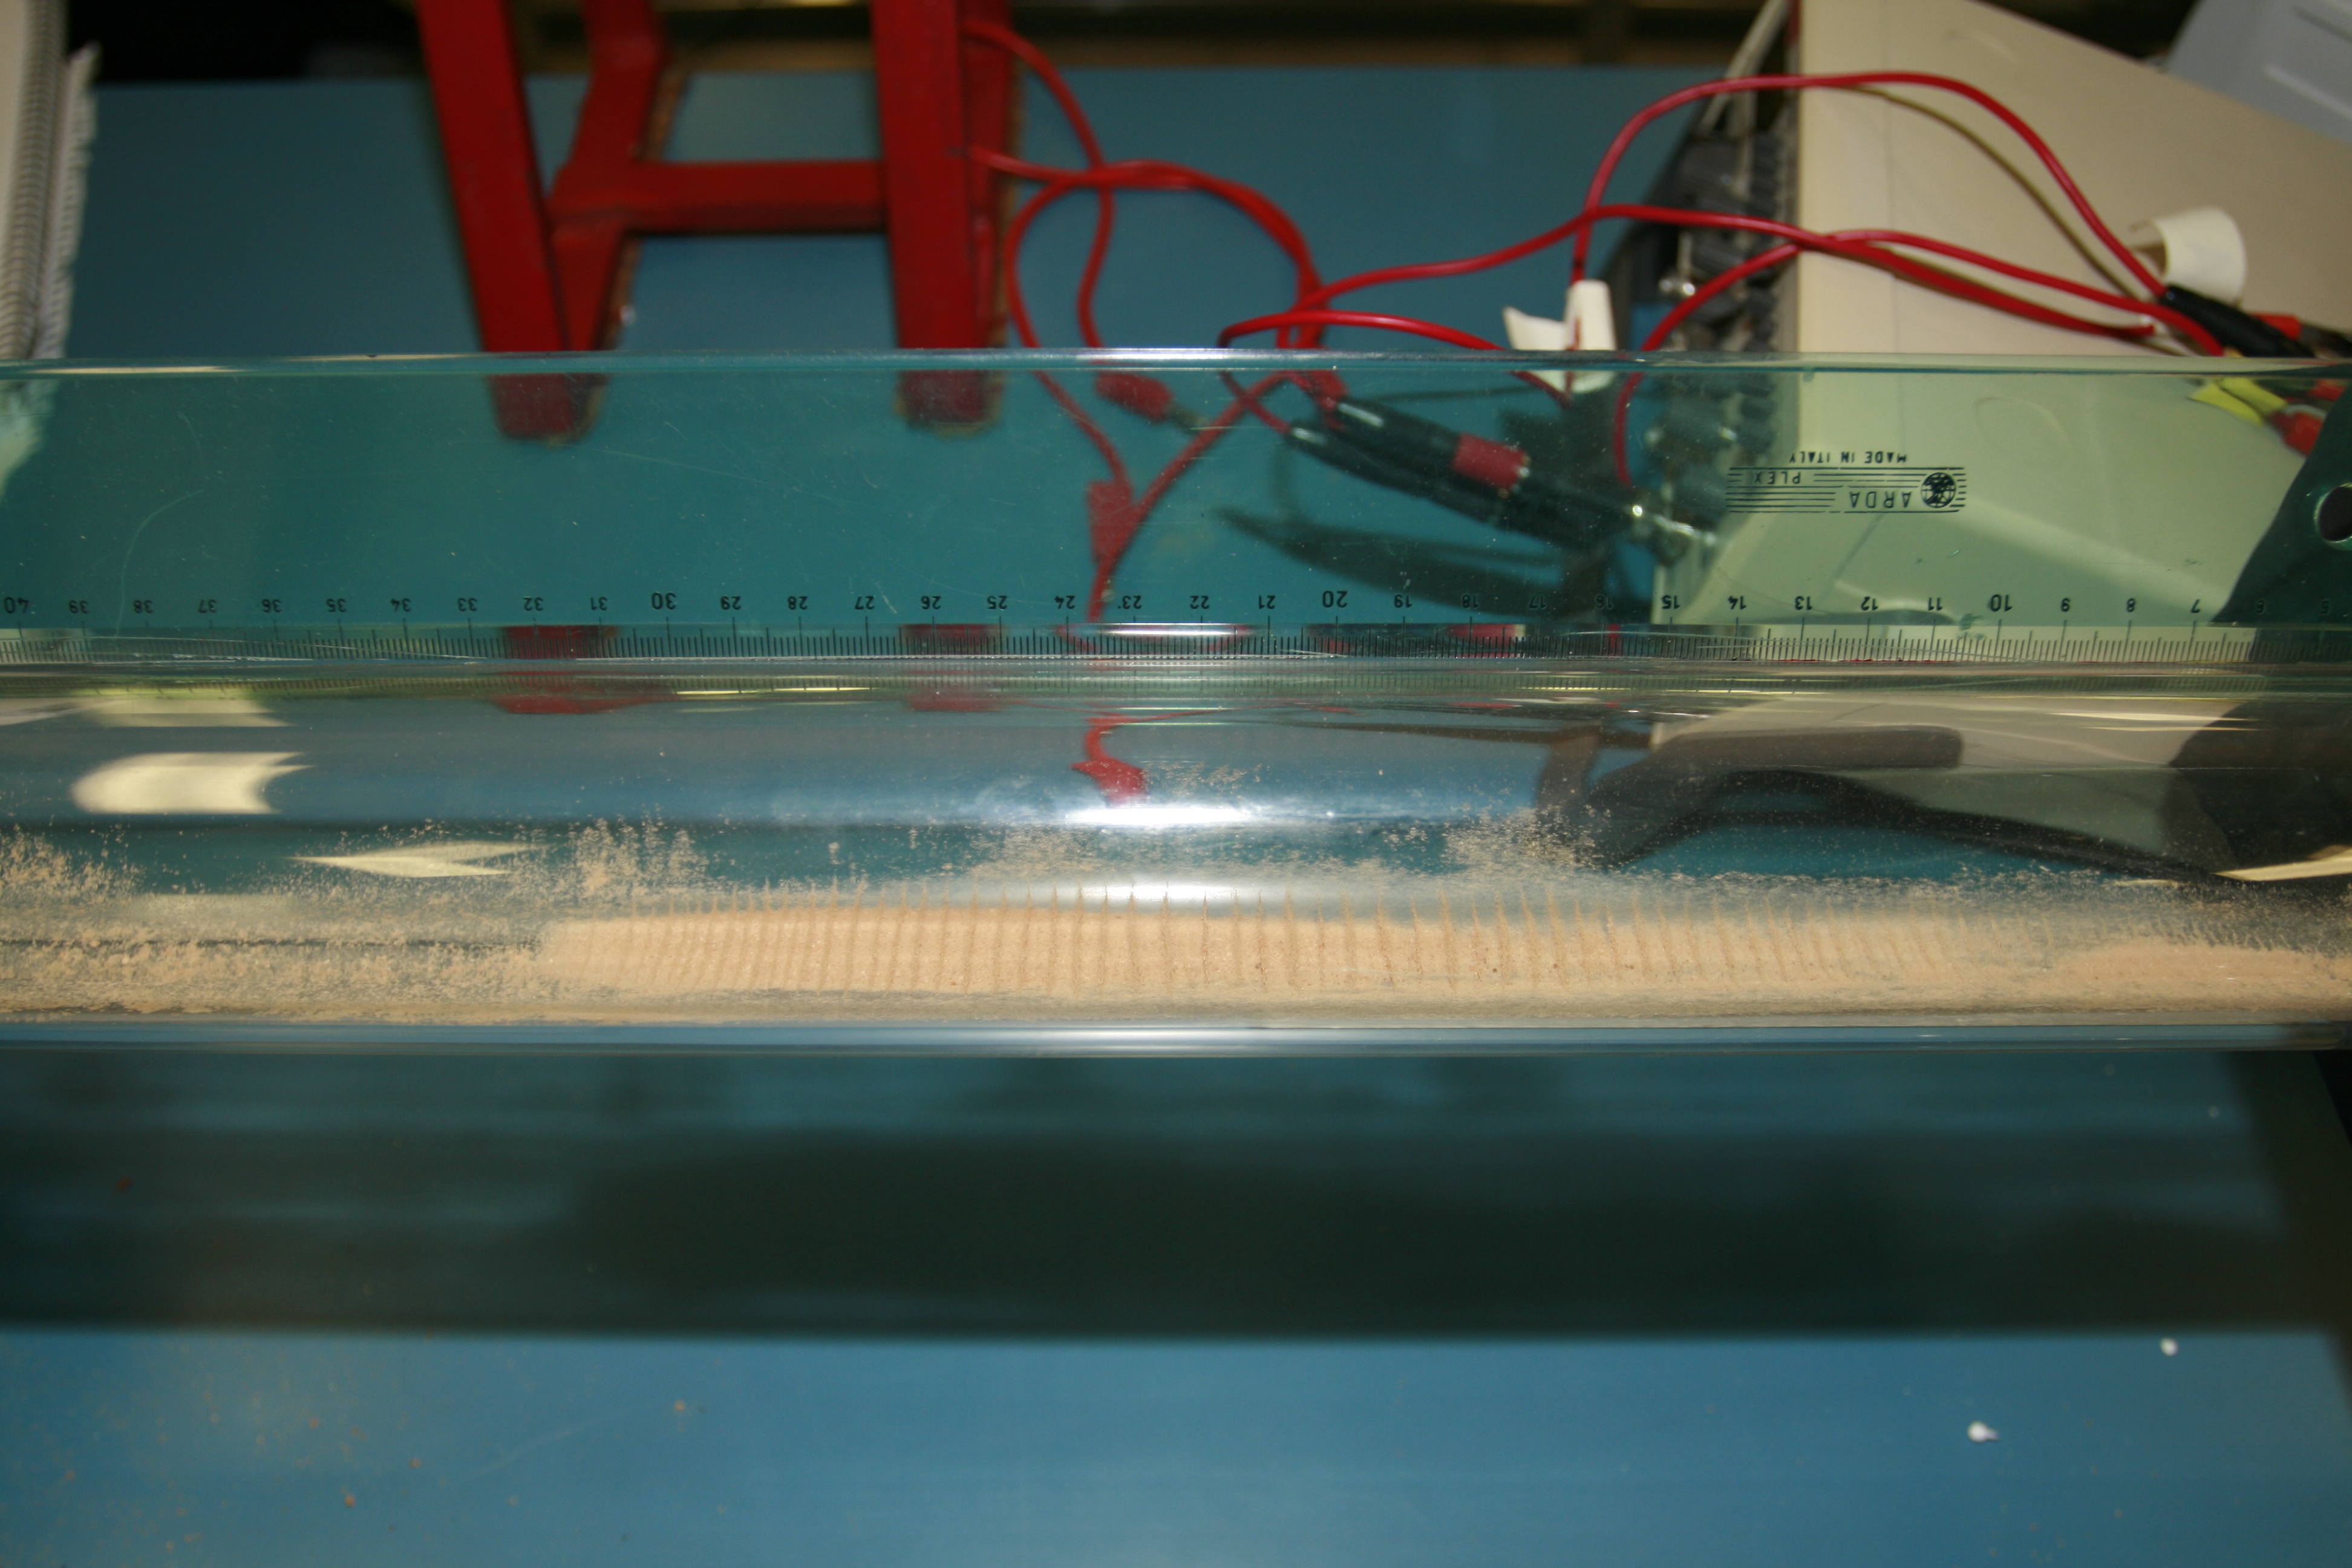
\includegraphics[width=\textwidth]{../Immagini/nodi_ventri.png}
 % striature_1.png: 2145x577 pixel, 400dpi, 13.63x3.67 cm, bb=
 \caption{In prossimità dei nodi la polvere è immobile e l'ampiezza di oscillazione delle molecole d'aria non è sufficiente a mantenere i muri di polvere che possiamo osservare in prossimità dei ventri}
 \label{fig:striature_ventri}
\end{figure}


\section*{Descrizione della strumentazione}

\subsection*{Specchio di LLoyd}

Per questo esperimento utilizzeremo una coppia di trasduttori in configurazione ricevitore-trasmettitore (r-t) 400ST160/400SR160 montati su due sopporti di legno. L'emettitore dovrà essere, per quanto possibile, allineato al ricevitore mentre lo specchio verrà allineato all'asse r-t. Sarà vostra premura assicurare che i trasduttori siano posizionati simmetricamente rispetto al centro dello specchio. Per chi fosse interessato alle caratteristiche fisiche dei trasduttori ultrasonici il \emph{datasheet} del produttore è disponibile sulla pagina del laboratorio di acustica all'indirizzo \url{cartan.e-moka.net}

\begin{figure}[H]
 \centering
 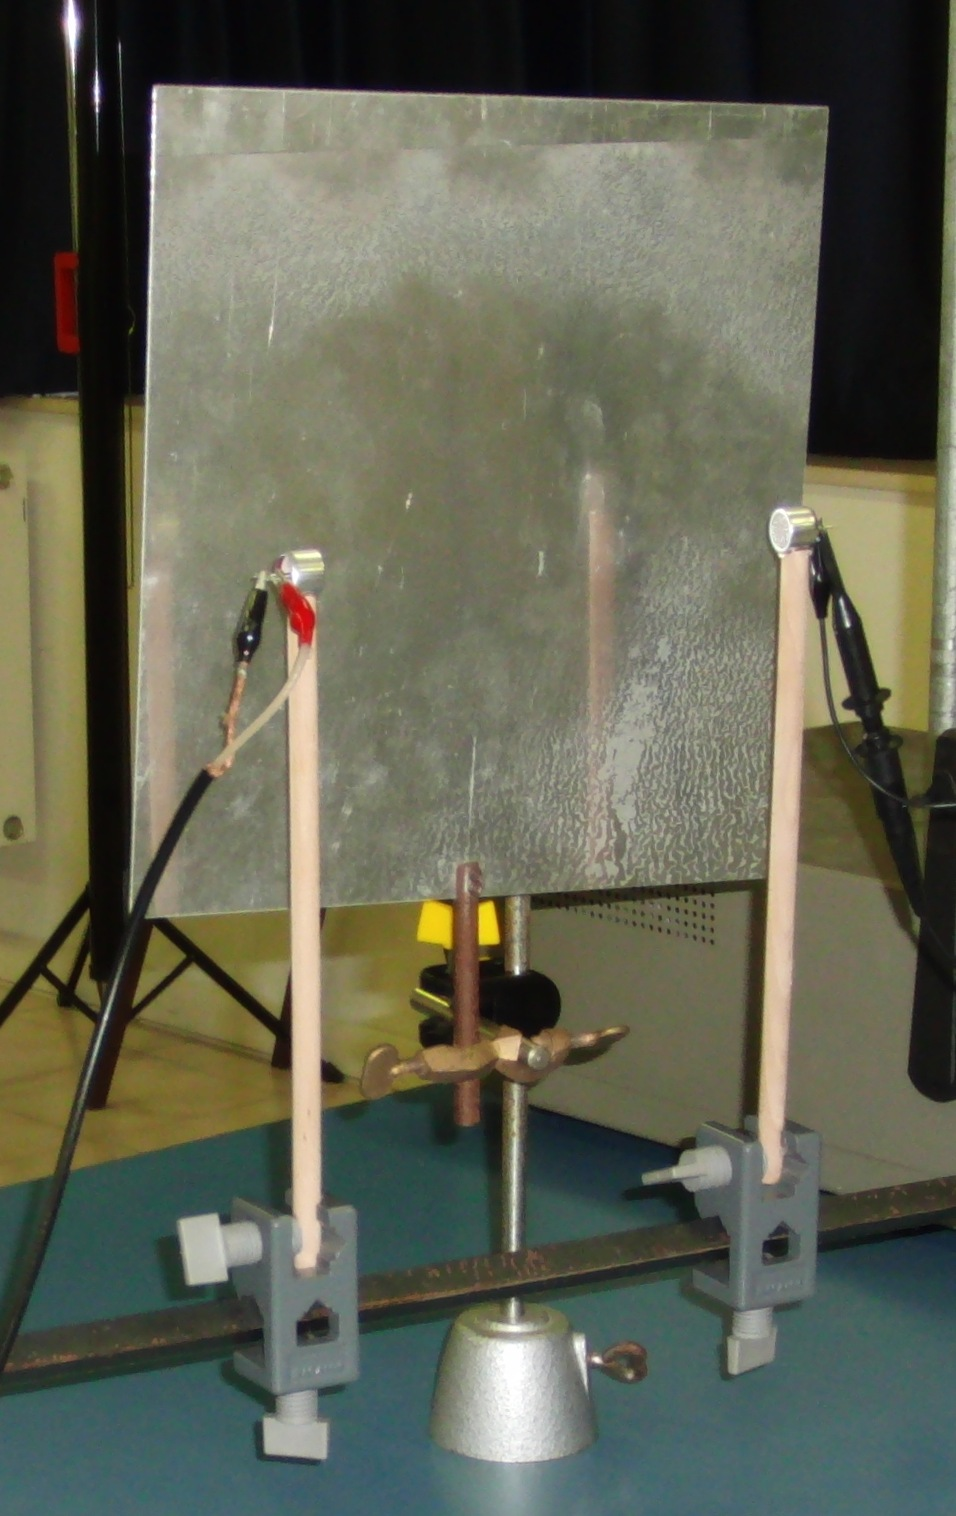
\includegraphics[width=0.5\textwidth]{../Immagini/specchio_llody.JPG}
 % specchio_llody.JPG: 956x1516 pixel, 72dpi, 33.73x53.48 cm, bb=0 0 956 1516
 \label{fig:specchio_llody_lab}
\end{figure}


\subsection*{Interferenza e diffrazione}
Per questo esperimento utilizzeremo una coppia di trasduttori in configurazione ricevitore-trasmettitore (r-t) 400ET160/400ER160 montati su due sopporti di legno. L'emettitore dovrà essere, per quanto possibile, allineato al ricevitore e all'ostacolo (doppia fenditura o singola fenditura). Sarà vostra premura assicurare che i trasduttori siano posizionati in modo da poter applicare le semplificazioni esposte precedentemente. Vi invitiamo ad osservare come cambiano le figure di interferenza e di diffrazione al variare delle posizioni di ricevitore ed emettitore rispetto all'ostacolo. Per chi fosse interessato alle caratteristiche fisiche dei trasduttori ultrasonici il \emph{datasheet} del produttore è disponibile sulla pagina del laboratorio di acustica all'indirizzo \url{cartan.e-moka.net}
\begin{figure}[H]
 \centering
 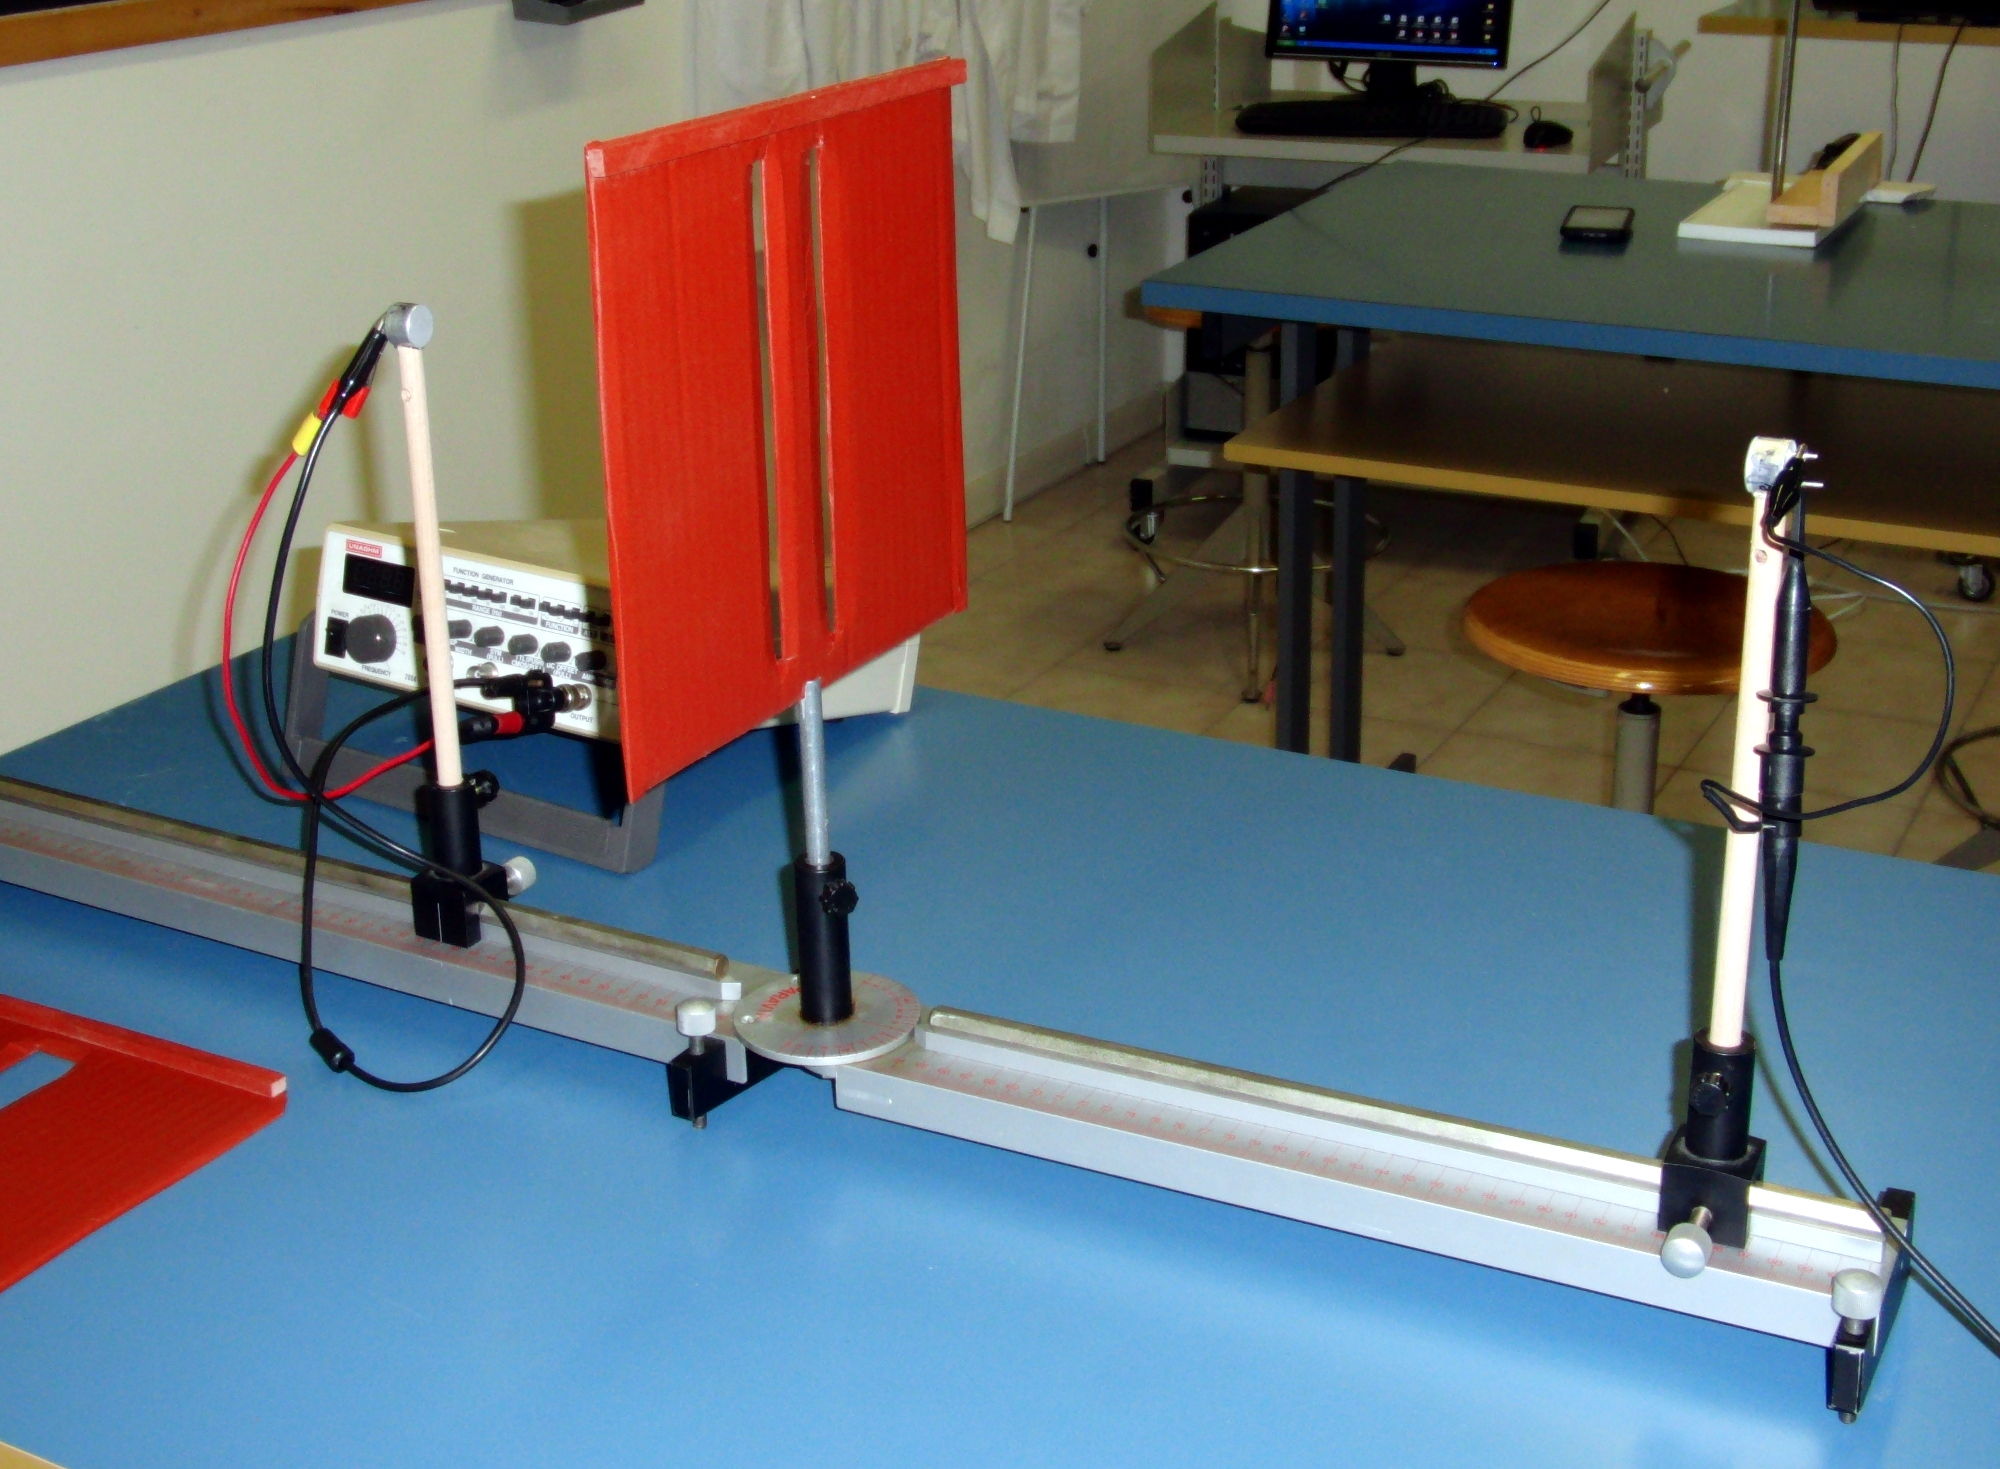
\includegraphics[width=0.8\textwidth]{../Immagini/young.JPG}
 % young.JPG: 2000x1469 pixel, 72dpi, 70.56x51.82 cm, bb=0 0 2000 1469
 \label{fig:young}
\end{figure}



\subsection*{Tubo opaco}

Il tubo è in cartone nero  corredato da un pistone con  microfono per variarne la lunghezza. Il microfono è stato ricavato da un vecchio microfono per computer ed il pistone è stato realizzato in gesso. Durante l'esperimento dovrete posizionare l'altoparlante in corrispondenza della bocca del tubo avendo cura di non occludere eccessivamente la stessa.


\begin{figure}[H]
 \centering
 \includegraphics[width=0.4\textwidth]{../Immagini/pistone.jpg}
 % pistone.jpg: 1804x1948 pixel, 72dpi, 63.64x68.72 cm, bb=0 0 1804 1948
 \caption{Il pistone mobile è stato costruito in gesso e al suo interno è stato inserito un microfono per campionare il fronte d'onda sonoro}
 \label{fig:pistone}
\end{figure}


\begin{figure}[H]
 \centering
 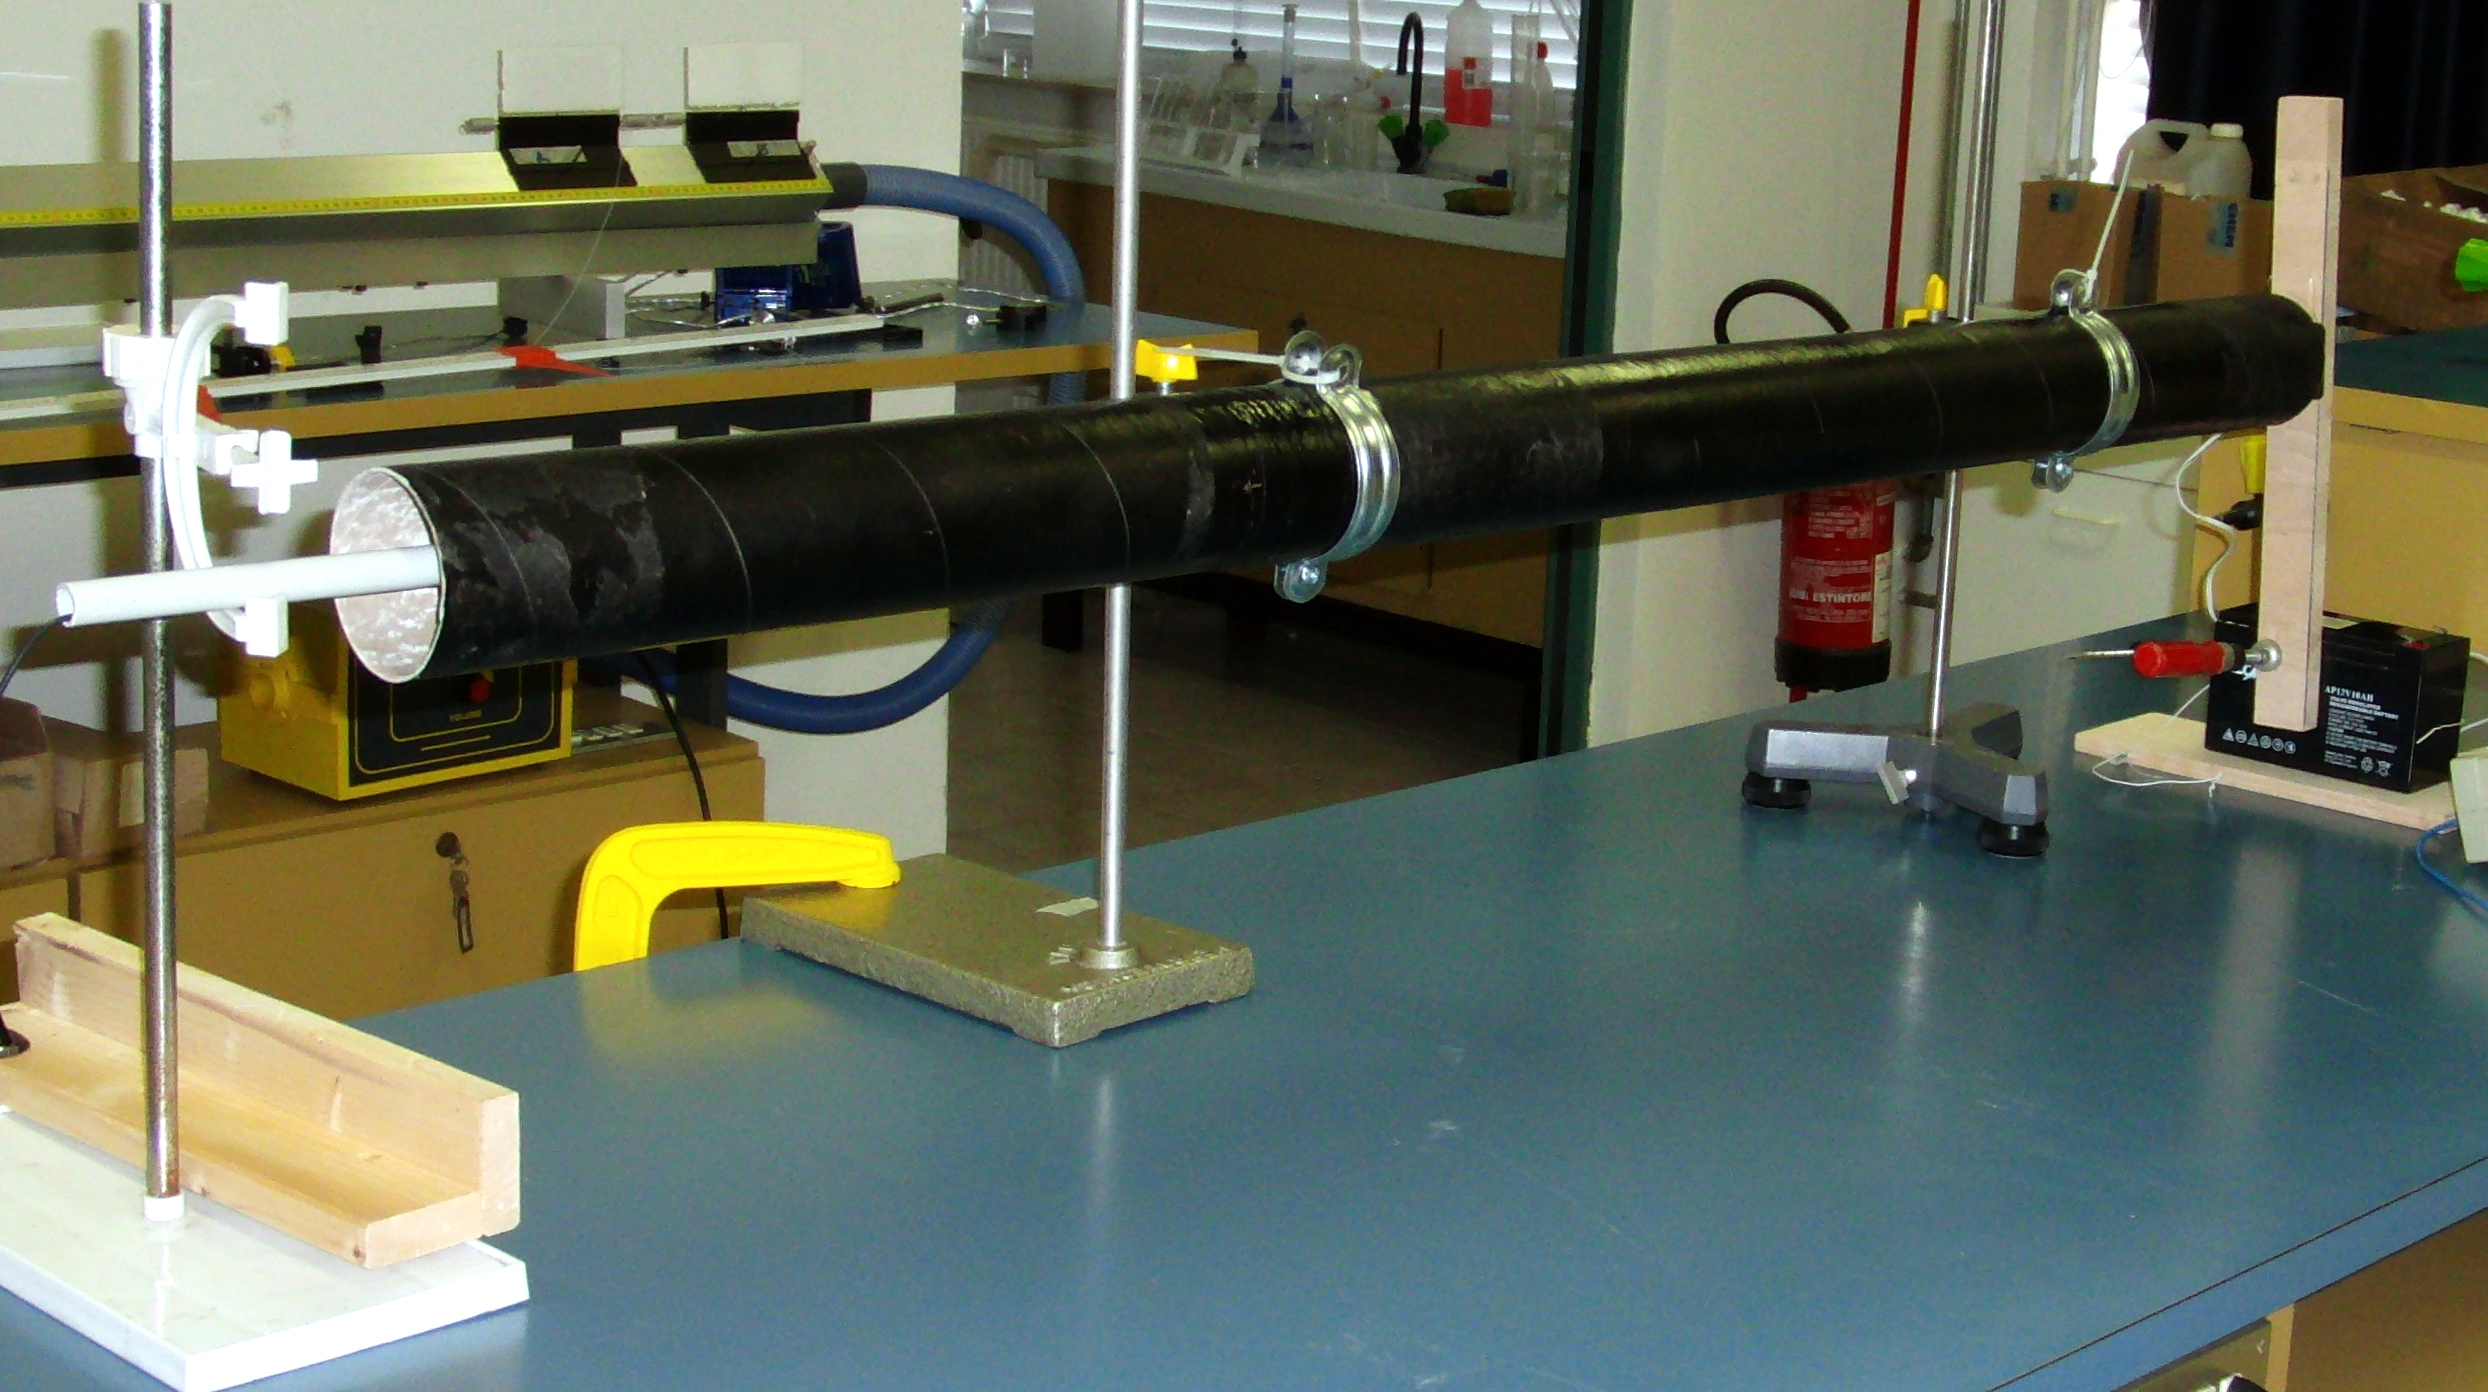
\includegraphics[width=\textwidth]{../Immagini/tubo_nero.JPG}
 % tubi_cartone.jpg: 3332x1090 pixel, 72dpi, 117.55x38.45 cm, bb=
 \caption{Tubo opaco in cartone come da laboratorio 2010/2011}
 \label{fig:tubi_cartone}
\end{figure}


\subsection*{Tubo trasparente}

Il tubo in plexiglas è dotato di tappo e di un imbuto per convogliare le onde sonore, a causa di fenomeni elettrostatici vi consigliamo di spruzzare su un panno dello spray anti-polvere e con questo pulire le pareti interne del tubo prima di effettuare l'esperimento.



\begin{figure}[H]
 \centering
 \includegraphics[width=\textwidth]{../Immagini/tubo_kundt.JPG}
 % tubo_plexiglass.jpg: 2838x1255 pixel, 72dpi, 100.12x44.27 cm, bb=
 \caption{Tubo in plexiglass per l'osservazione delle striature nella polvere}
 \label{fig:tubo_plexiglass}
\end{figure}


\subsection*{Casse, amplificatori e trasduttori}

\begin{itemize}
 \item Una cassa da $15W$ con impedenza di $8\Omega$
 \item Una cassa da $4W$ con impedenza di $4\Omega$
 \item Un amplificatore in classe D (Yamaha D138) con una potenza RMS di $10W$ per canale
 \item Una coppia di trasduttori ultrasonici in configurazione ricevitore emettitore 400ST160/400SR160, una coppia di trasduttori ultrasonici  in configurazione emettitore ricevitore 400ET180/400ER180
\end{itemize}



\subsection*{Rilevatori e generatori}
\begin{itemize}
 \item 4 generatori di funzione
 \item 2 voltmetri ad alta precisione (da usarsi alternativamente agli oscilloscopi negli esperimenti con gli ultrasuoni)
 \item 2 oscilloscopi analogici da $20Mhz$
 \item 2 oscilloscopi digitali con analizzatore di frequenza simulati tramite computer e scheda sonora con il programma Zelscope (in  Gnu/Linux potete usare Xoscope)
\end{itemize}

\section*{Attività di laboratorio}
Vediamo ora nel dettaglio le attività che svolgeremo in laboratorio iniziando dalla misura della velocità del suono.

\subsection*{Misura della velocità del suono}
Per tale misura utilizzeremo i tubi in cartone e le casse non amplificate. Per prima cosa posizioneremo una cassa in prossimità di un'apertura del tubo ed inseriremo il pistone in quella opposta, quindi genereremo una frequenza sostenibile dalla cassa che misureremo accuratamente utilizzando l'oscilloscopio software. Dopo aver effettuato questi preparativi il sistema è pronto per le misure da eseguire in questo ordine:
\begin{itemize}
 \item Impostiamo l'oscilloscopio digitale in modalità analizzatore di spettro
 \item Spostiamo il pistone lungo il tubo fino ad incontrare una risonanza e riportiamo sul gambo dello stesso una tacca
 \item Ripetiamo il passo precedente fino ad estrarre il pistone dal tubo
 \item Misuriamo le distanze tra le tacche 
 \item Riportiamo in una tabelle la lista delle distanze misurate e la frequenza del suono
\item Ripetiamo tutta la procedura (compresa l'impostazione iniziale) per una frequenza diversa
\end{itemize}
Tutto il procedimento sopra descritto dovrebbe essere ripetuto per almeno tre frequenze diverse.

\subsection*{Misura della lunghezza acustica del tubo}

Come sappiamo dalla teoria i tubi (e gli strumenti musicali a colonna d'aria) si comportano come se fossero leggermente più lunghi, quando andiamo a calcolare le frequenze di risonanza. Vogliamo misurare di quanto dobbiamo correggere le nostre formule in funzione del diametro del tubo. Procederemo in questo modo:
\begin{itemize}
 \item Posizioniamo il pistone ad una distanza $L$ dall'estremo aperto del tubo e misuriamone accuratamente il valore
 \item Calcoliamo con la formula studiata un'armonica superiore per tale lunghezza del tubo (dobbiamo usare una frequenza abbastanza alta dato che le casse presenti in laboratorio non riproducono fedelmente le basse frequenze ad esempio possiamo usare la terza armonica oppure scegliere una $L$ sufficientemente piccola)
 \item Variando la frequenza in un intorno di quella calcolata cerchiamo la risonanza tramite l'analizzatore di spettro  e misuriamo accuratamente tale frequenza con l'oscilloscopio software del computer. La frequenza risonante dovrebbe essere più piccola di quella calcolata dato che il tubo è, dal punto di vista acustico, leggermente più lungo
\item Calcoliamo la lunghezza di risonanza teorica corrispondente a tale frequenza
\item Sottraiamo la lunghezza reale $L$ misurata alla $L^*$ precedentemente calcolata per determinare la correzione $\delta$.
\end{itemize}
Tutto il procedimento va ripetuto per almeno tre lunghezze diverse, potete trascrivere le vostre misure come in tabella  [\ref{tab:correzione}].

\begin{table}[H]
\begin{center}
\begin{tabular}{llll}\toprule
$\nu_{risonanza}$ &$L$&$L^*$&$L^*-L$\\ \midrule
142Hz & 10cm &12.1cm&2.1cm\\
425Hz & 6cm  &8.3cm&2.3cm\\
568Hz & 3cm  &5.2cm&2.2cm\\
\ldots &\ldots&\ldots&\ldots \\ \bottomrule
\end{tabular}\caption{I dati in tabella \textbf{non} sono rappresentativi di una misura reale e dovranno essere utilizzati unicamente come guida per la tabulazione delle misure da voi effettuate}\label{tab:correzione}
\end{center}
\end{table}


\subsection*{Misura delle distanze tra le striature della polvere di sughero nei tubi trasparenti}

Il tubo trasparente e la polvere di sughero ci permettono una interessante visualizzazione delle onde stazionarie che si generano al suo interno. L'esperimento ci permetterà di osservare anche le caratteristiche striature che si formano quando la colonna d'aria è  in risonanza.
Procedimento:
\begin{itemize}
 \item Misuriamo la lunghezza ed il diametro del tubo
 \item Disponiamo con l'apposito strumento un leggero velo di polvere lungo il tubo
 \item Disponiamo l'imbuto sull'imboccatura ed accostiamo la cassa.
 \item Cerchiamo la frequenza di risonanza del tubo (difficilmente si potrà osservare l'armonica fondamentale a causa delle caratteristiche meccaniche delle casse)
 \item Trascriviamo ogni frequenza di risonanza e fotografiamo le striature che si vengono a formare.

\end{itemize}

Tutto il procedimento va ripetuto sia con tubo semichiuso che con tubo aperto.
\begin{figure}[H]
 \centering
 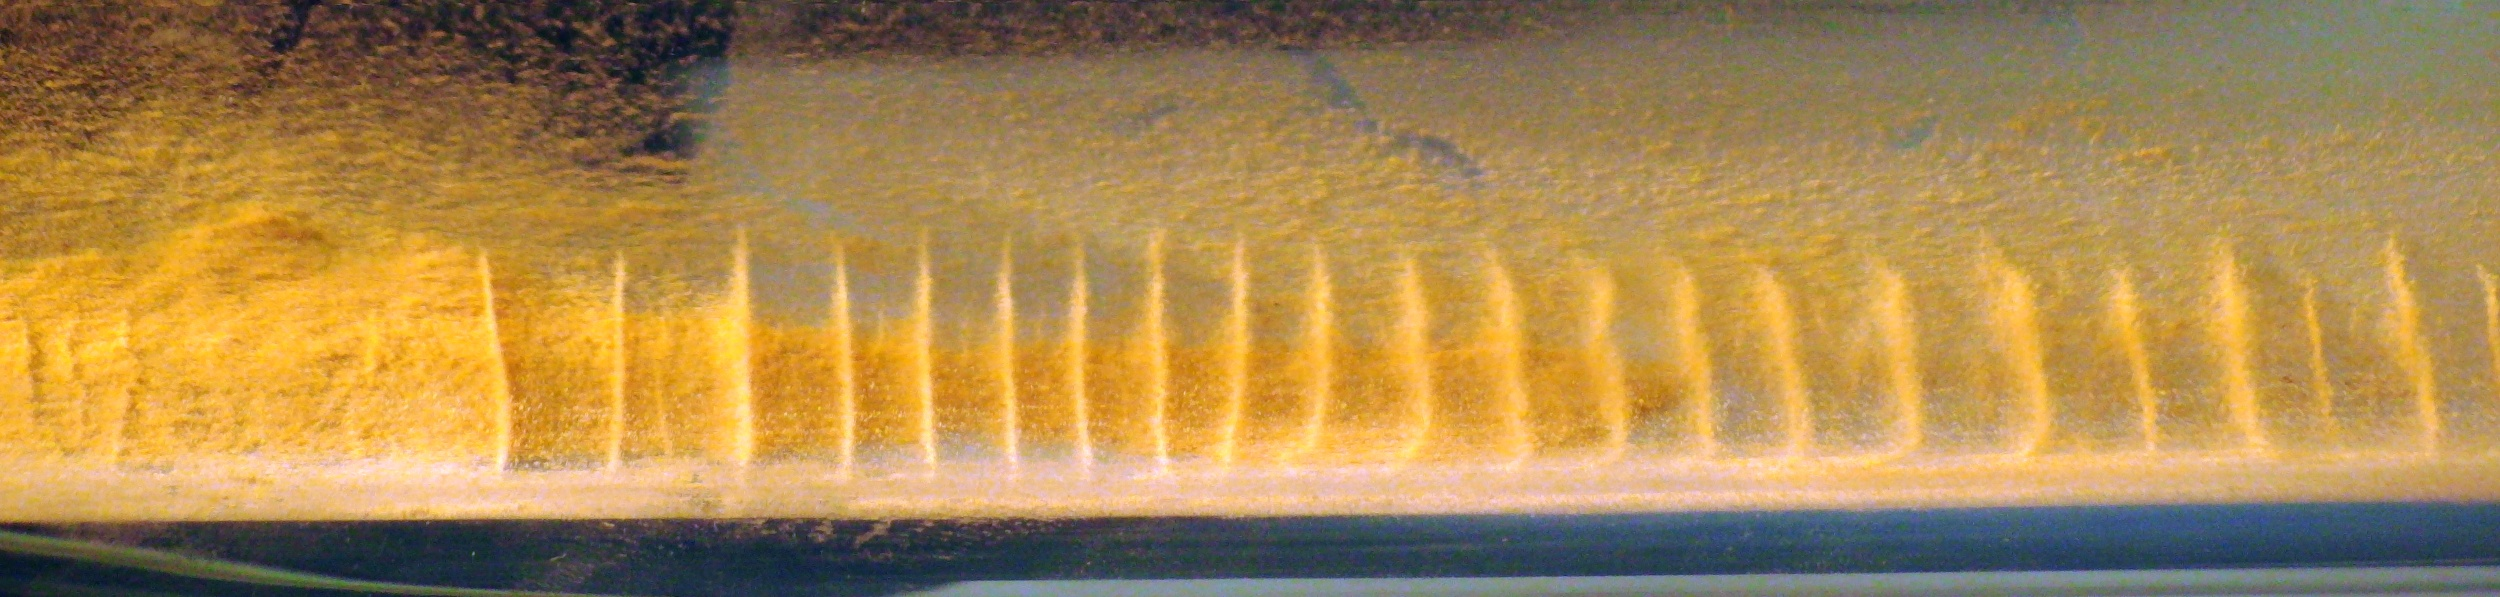
\includegraphics[width=\textwidth]{../Immagini/fondo_strie.jpg}
 % striature1.jpg: 2486x616 pixel, 72dpi, 87.70x21.73 cm, bb=
 \caption{Striature nella polvere di sughero all'insorgere di una risonanza nella colonna d'aria all'interno del tubo di plexiglass.}
 \label{fig:striature1}
\end{figure}

\section*{Misura di interferenza con lo specchio di LLoyd}

In questo esperimento sposteremo lo specchio perpendicolarmente all'asse di ricevitore e trasmettitore (r-t) per variare la posizione della sorgente virtuale e quindi l'ampiezza dell'onda misurata dal ricevitore. Opereremo utilizzando la procedure seguente:
\begin{itemize}
 \item Posizioniamo lo specchio metallico ad una distanza nota dall'asse r-t ad esempio a ridosso dell'armatura metallica dei trasduttori
\item Misuriamo la distanza $d$ dello specchio dall'asse r-t
\item Misuriamo l'ampiezza in volt del segnale raccolto dall'oscilloscopio
\item Ripetiamo la misura variando di volta in volta la distanza $d$ 
\end{itemize}

Per ottenere una buona stima delle posizioni dei minimi e dei massimi e quindi confrontarle con i risultati teorici [\ref{llody_dmin}] e [\ref{lloyd_dmax}] dobbiamo usare un passo spaziale dell'ordine del millimetro  soprattutto in prossimità del cambiamento di pendenza della curva. Dopo aver tabulato i dati questi dovranno essere utilizzati per rappresentare la curva $V(d)$ ovvero il voltaggio misurato in funzione della distanza $d$, per tale compito potete utilizzare il foglio di calcolo oppure uno dei software proposti nei laboratori degli scorsi anni come Scilab, Octave o Gnuplot.


\begin{figure}[H]
 \centering
 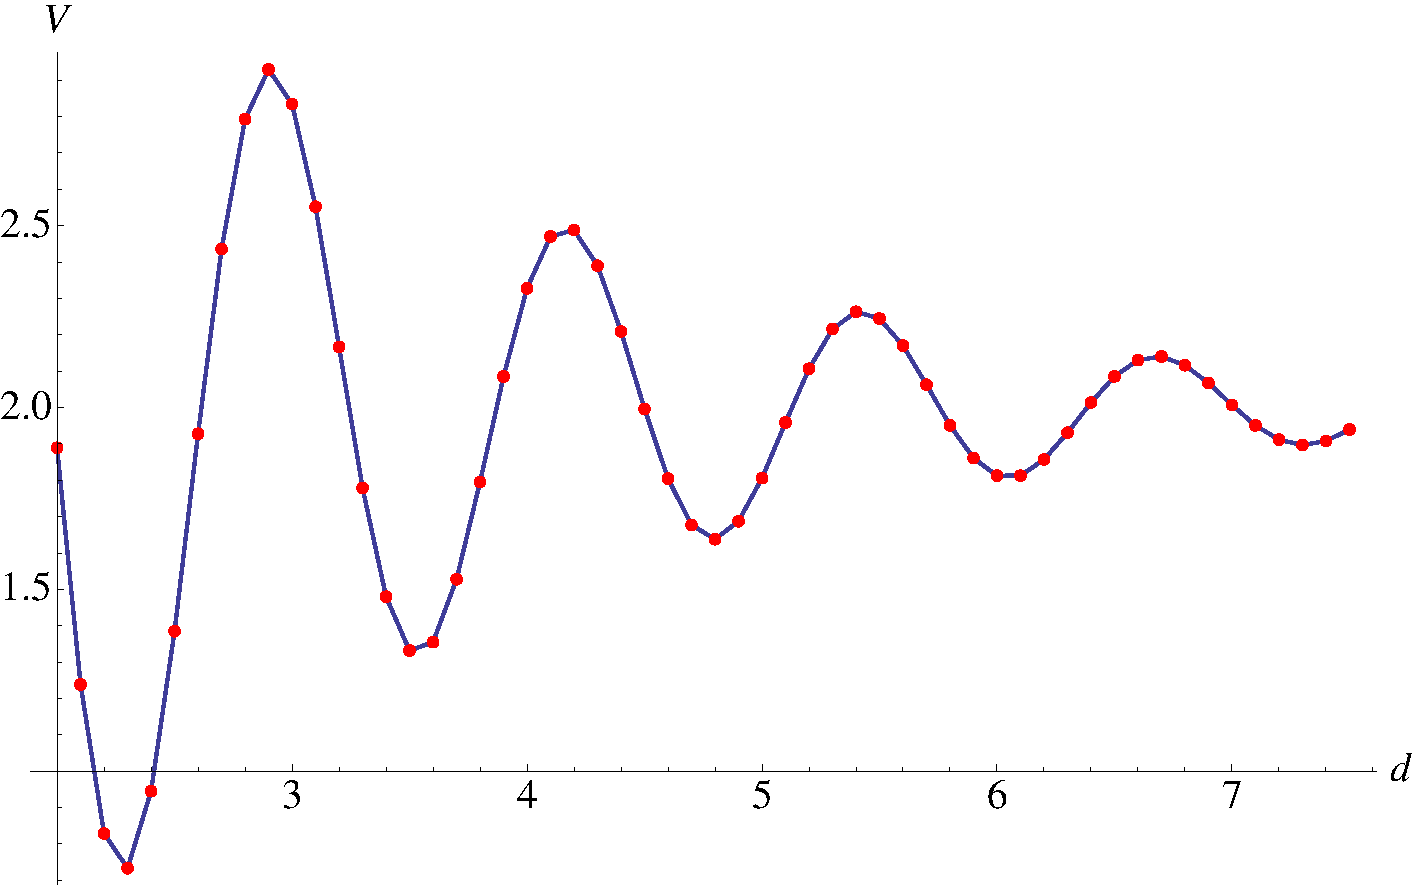
\includegraphics[width=0.8\textwidth]{../Immagini/esempio_misura_lloyd.pdf}
 % esempio_misura_lloyd.pdf: 706x442 pixel, 72dpi, 24.91x15.59 cm, bb=0 0 706 442
 \caption{Risultato della misura in condizioni ideali è stato usata un passo fisso pari a $\Delta d=1mm$ tra le misure. I dati sono puramente indicativi}
 \label{fig:misura_llody}
\end{figure}



\section*{Esperimento di Young acustico}

Per la misura della figura di interferenza prodotta da due fenditure illuminate da una sorgente di ultrasuoni procederemo nel modo seguente:

\begin{itemize}
 \item Posizioniamo lo schermo in modo che l'occlusione si trovi allineata all'asse r-t
 \item Variamo la posizione angolare del braccio libero del supporto e registriamo il corrispondente valore di tensione indicato dall'oscilloscopio
\item Ripetiamo il procedimento per quante più posizioni angolari possibili
\end{itemize}
Dopo aver raccolto e tabulato i dati realizzerete con essi un grafico, il risultato di tale operazione dovrebbe essere simile a figura [\ref{fig:esempio_young}]

\begin{figure}[H]
 \centering
 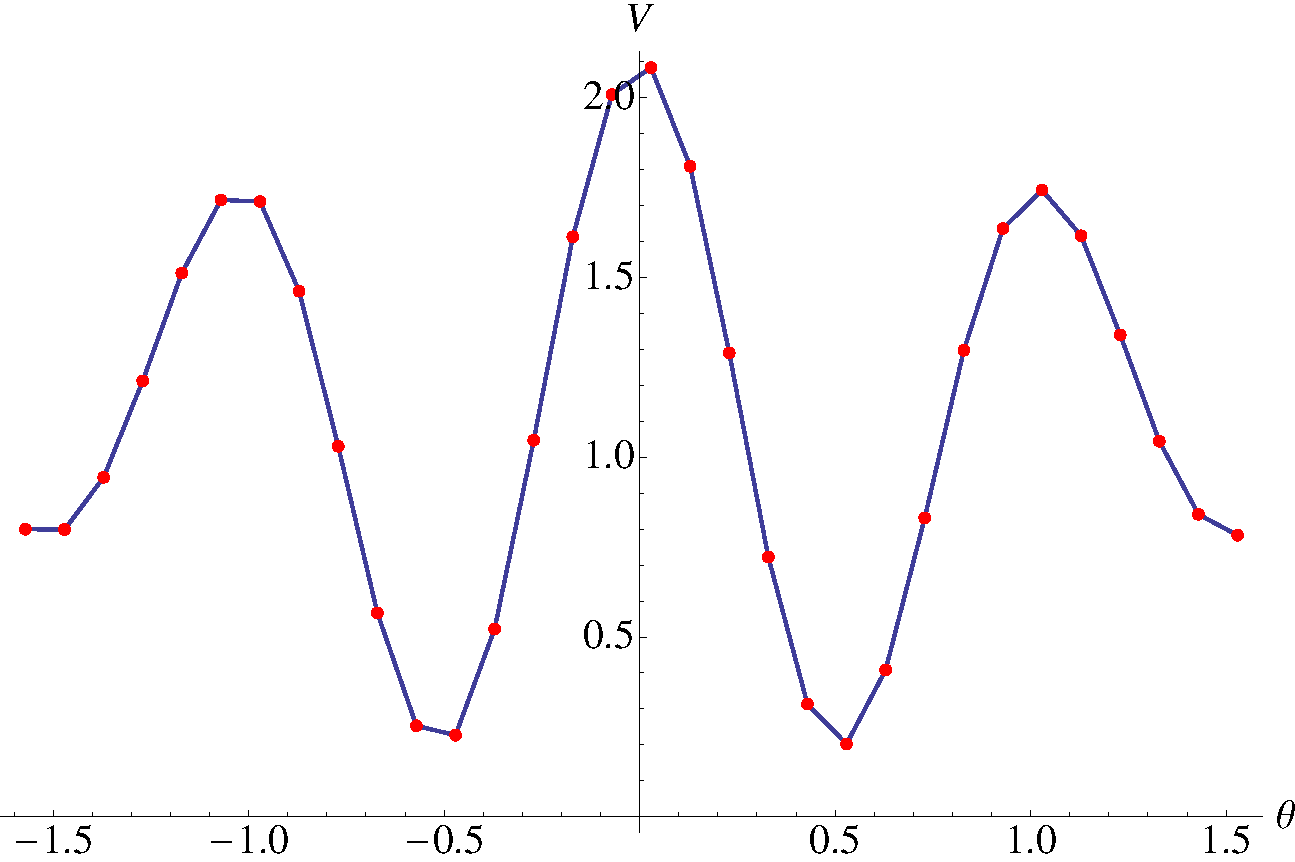
\includegraphics[width=0.8\textwidth]{../Immagini/esempio_misura_young.pdf}
 % esempio_misura_young.pdf: 622x414 pixel, 72dpi, 21.94x14.60 cm, bb=0 0 622 414
 \caption{Nella misura dell'interferenza da due fenditure riporteremo sull'asse delle ascisse l'ampiezza in radianti dell'angolo e sull'asse delle ordinate il voltaggio misurato dall'oscilloscopio. I dati sono puramente indicativi}
 \label{fig:esempio_young}
\end{figure}


\section*{Diffrazione di un'onda ultrasonica da una fenditura rettangolare}
Per la misura della figura di diffrazione, prodotta da una fenditura di larghezza maggiore alla lunghezza d'onda del suono, illuminata da una sorgente di ultrasuoni, procederemo nel modo seguente:

\begin{itemize}
 \item Posizioniamo lo schermo in modo che il centro dell'apertura si trovi allineato all'asse r-t
 \item Variamo la posizione angolare del braccio libero del supporto e registriamo il corrispondente valore di tensione indicato dall'oscilloscopio
 \item Ripetiamo il procedimento per quante più posizioni angolari possibili
\end{itemize}
Dopo aver raccolto e tabulato i dati realizzerete con essi un grafico, il risultato di tale operazione dovrebbe essere simile a figura [\ref{fig:fraun_misura}]

\begin{figure}[H]
 \centering
 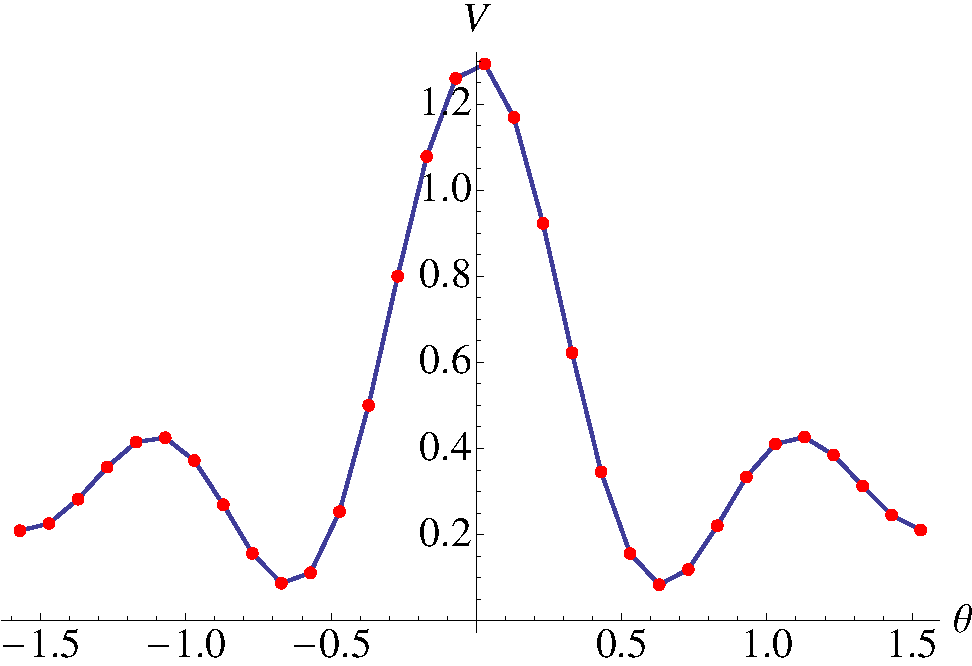
\includegraphics[width=0.8\textwidth]{../Immagini/esempio_misura_fraun.pdf}
 % esempio_misura_fraun.pdf: 466x320 pixel, 72dpi, 16.44x11.29 cm, bb=0 0 466 320
 \caption{Esempio di misura dell'intensità dell'onda difratta dalla singola fenditura in funzione dell'angolo di diffrazione. I dati sono puramente indicativi.}
 \label{fig:fraun_misura}
\end{figure}

\end{document}
